 

\documentclass[12pt]{article}
%%%%%%%%%%%%%%%%%%%%%%%%%%%%%%%%%%%%%%%%%%%%%%%%%%%%%%%%%%%%%%%%%%%%%%%%%%%%%%%%%%%%%%%%%%%%%%%%%%%%%%%%%%%%%%%%%%%%%%%%%%%%%%%%%%%%%%%%%%%%%%%%%%%%%%%%%%%%%%%%%%%%%%%%%%%%%%%%%%%%%%%%%%%%%%%%%%%%%%%%%%%%%%%%%%%%%%%%%%%%%%%%%%%%%%%%%%%%%%%%%%%%%%%%%%%%
\usepackage{amsfonts}
\usepackage{eurosym}
\usepackage{geometry}
\usepackage{amsmath,amsthm,amssymb}
\usepackage{graphicx}
\usepackage{comment}
\usepackage{adjustbox}
\usepackage{array}
\usepackage{multirow}
\usepackage{subcaption}
\usepackage{pifont}
\usepackage{amssymb}
\usepackage{comment}
\usepackage[utf8]{inputenc}
\usepackage{setspace}
\usepackage[hang, flushmargin, bottom]{footmisc}
%\usepackage[backend=biber,style=apa,url=false,isbn=false, extra = false]{biblatex}

%\addbibresource{references.bib}
\usepackage{footnotebackref}
\usepackage{xcolor}
\usepackage{hyperref}
\usepackage{booktabs}
\usepackage{pifont}
\usepackage{caption}
\usepackage{float}


\setlength{\textfloatsep}{5pt}
\captionsetup{font=normalsize}
\newcommand{\cmark}{\ding{51}}
\def\sym#1{\ifmmode^{#1}\else\(^{#1}\)\fi}
\renewcommand{\thetable}{\Roman{table}}
\geometry{verbose,tmargin=.5in,bmargin=.7in,lmargin=.7in,rmargin=.7in,nomarginpar}
\makeatletter

\begin{document}

\title{Initial empirical results from SCOMP data}

\maketitle

In this document I will present what we are learnign from out empirical work. This is the continuation of the file which presents the initial datawork. 

\section{IE 4}

\subsection{Elasticity of shoppers vs non-shoppers}

The following table shows the coefficients of a conditional logit to test whether customers that ask for an external offer are more price elastic. Odd (even) columns run the specification on the sample with(without) external offers, which we think of as shoppers (non-shoppers). Once we control by the company fixed effects the shopers are more elastic. 

\begin{table}[htbp]\centering
\def\sym#1{\ifmmode^{#1}\else\(^{#1}\)\fi}
\caption{Conditional Logit: Price Elasticity by External Offer Status}
\begin{tabular}{l*{6}{c}}
\hline\hline
            &\multicolumn{1}{c}{(1)}&\multicolumn{1}{c}{(2)}&\multicolumn{1}{c}{(3)}&\multicolumn{1}{c}{(4)}&\multicolumn{1}{c}{(5)}&\multicolumn{1}{c}{(6)}\\
            &\multicolumn{1}{c}{Has External}&\multicolumn{1}{c}{No External}&\multicolumn{1}{c}{Has External (FE)}&\multicolumn{1}{c}{No External (FE)}&\multicolumn{1}{c}{m5}&\multicolumn{1}{c}{m6}\\
\hline
accepted    &                     &                     &                     &                     &                     &                     \\
val\_uf\_pension1&       7.227\sym{***}&       7.924\sym{***}&       7.996\sym{***}&       7.689\sym{***}&                     &                     \\
            &     (0.077)         &     (0.192)         &     (0.082)         &     (0.210)         &                     &                     \\
[1em]
Nrisk       &       0.555\sym{***}&       0.284\sym{***}&       0.148\sym{***}&       0.254\sym{***}&       0.126\sym{***}&       0.283\sym{***}\\
            &     (0.010)         &     (0.012)         &     (0.033)         &     (0.046)         &     (0.037)         &     (0.049)         \\
[1em]
val\_uf\_pension\_z&                     &                     &                     &                     &       2.586\sym{***}&       2.077\sym{***}\\
            &                     &                     &                     &                     &     (0.022)         &     (0.039)         \\
\hline
\(N\)       &      207700         &       45580         &      207700         &       45580         &      207700         &       45568         \\
Log likelihood&   -26295.01         &    -7517.02         &   -24596.21         &    -7095.09         &   -18225.26         &    -6097.02         \\
Chi-squared &    20103.57         &     3677.36         &    23501.18         &     4521.20         &    36243.08         &     6509.03         \\
\hline\hline
\multicolumn{7}{l}{\footnotesize Standard errors in parentheses.}\\
\multicolumn{7}{l}{\footnotesize Models 1-2: Without firm fixed effects.}\\
\multicolumn{7}{l}{\footnotesize Models 3-4: With firm fixed effects.}\\
\multicolumn{7}{l}{\footnotesize *** p<0.01, ** p<0.05, * p<0.10}\\
\end{tabular}
\end{table}

 
 \subsection{Firms using more-less external offers}

\begin{figure}[H]
\caption{}
 \label{fig:ie4_1}
\centering{}%
\begin{tabular}{cc}
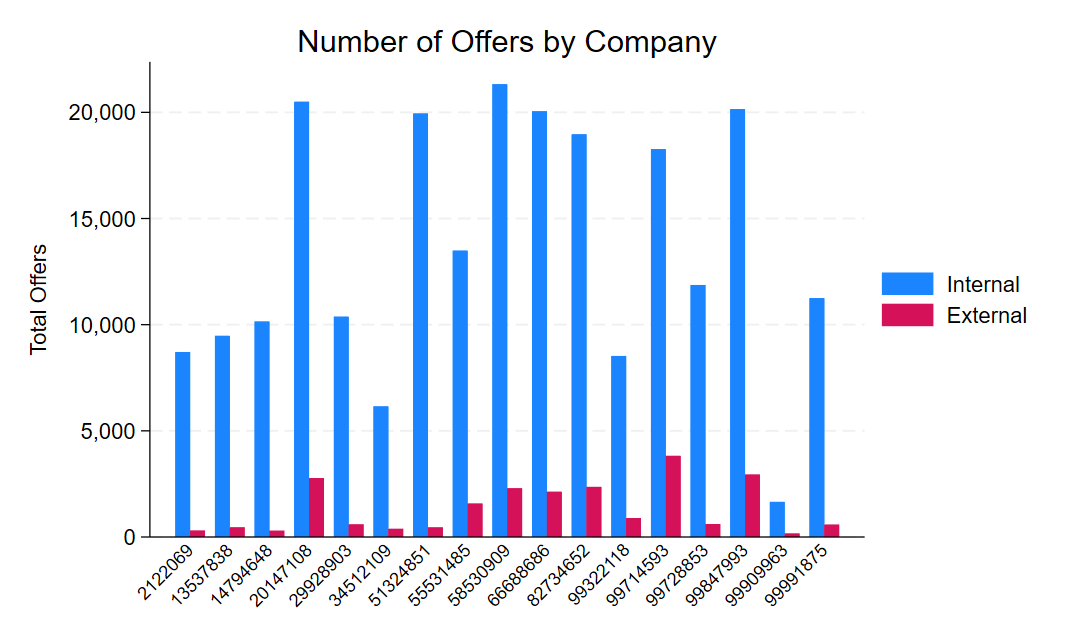
\includegraphics[scale=0.17]{../figures/IE4/IE4_int_ext_offers_by_cia.png} 
\end{tabular}
\end{figure}

\begin{figure}[H]
\caption{}
 \label{fig:ie4_2and3}
\centering{}%
\begin{tabular}{cc}
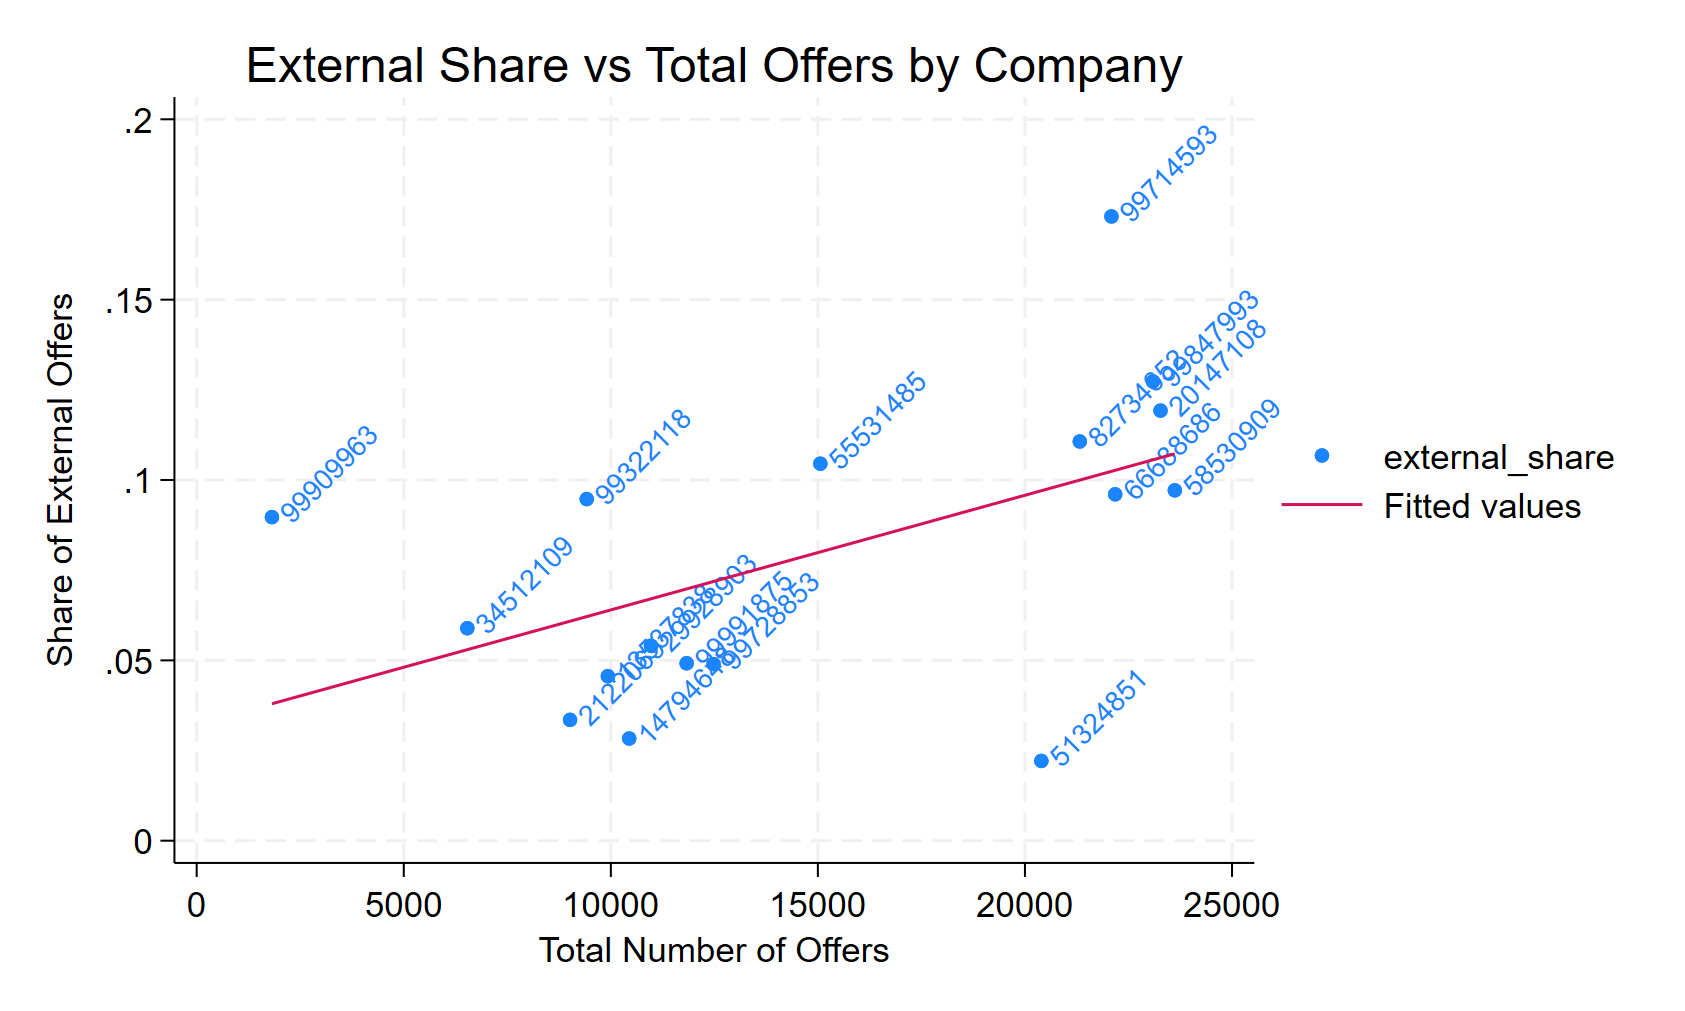
\includegraphics[scale=0.17]{../figures/IE4/IE4_total_internal_offers_bycompany.png} & 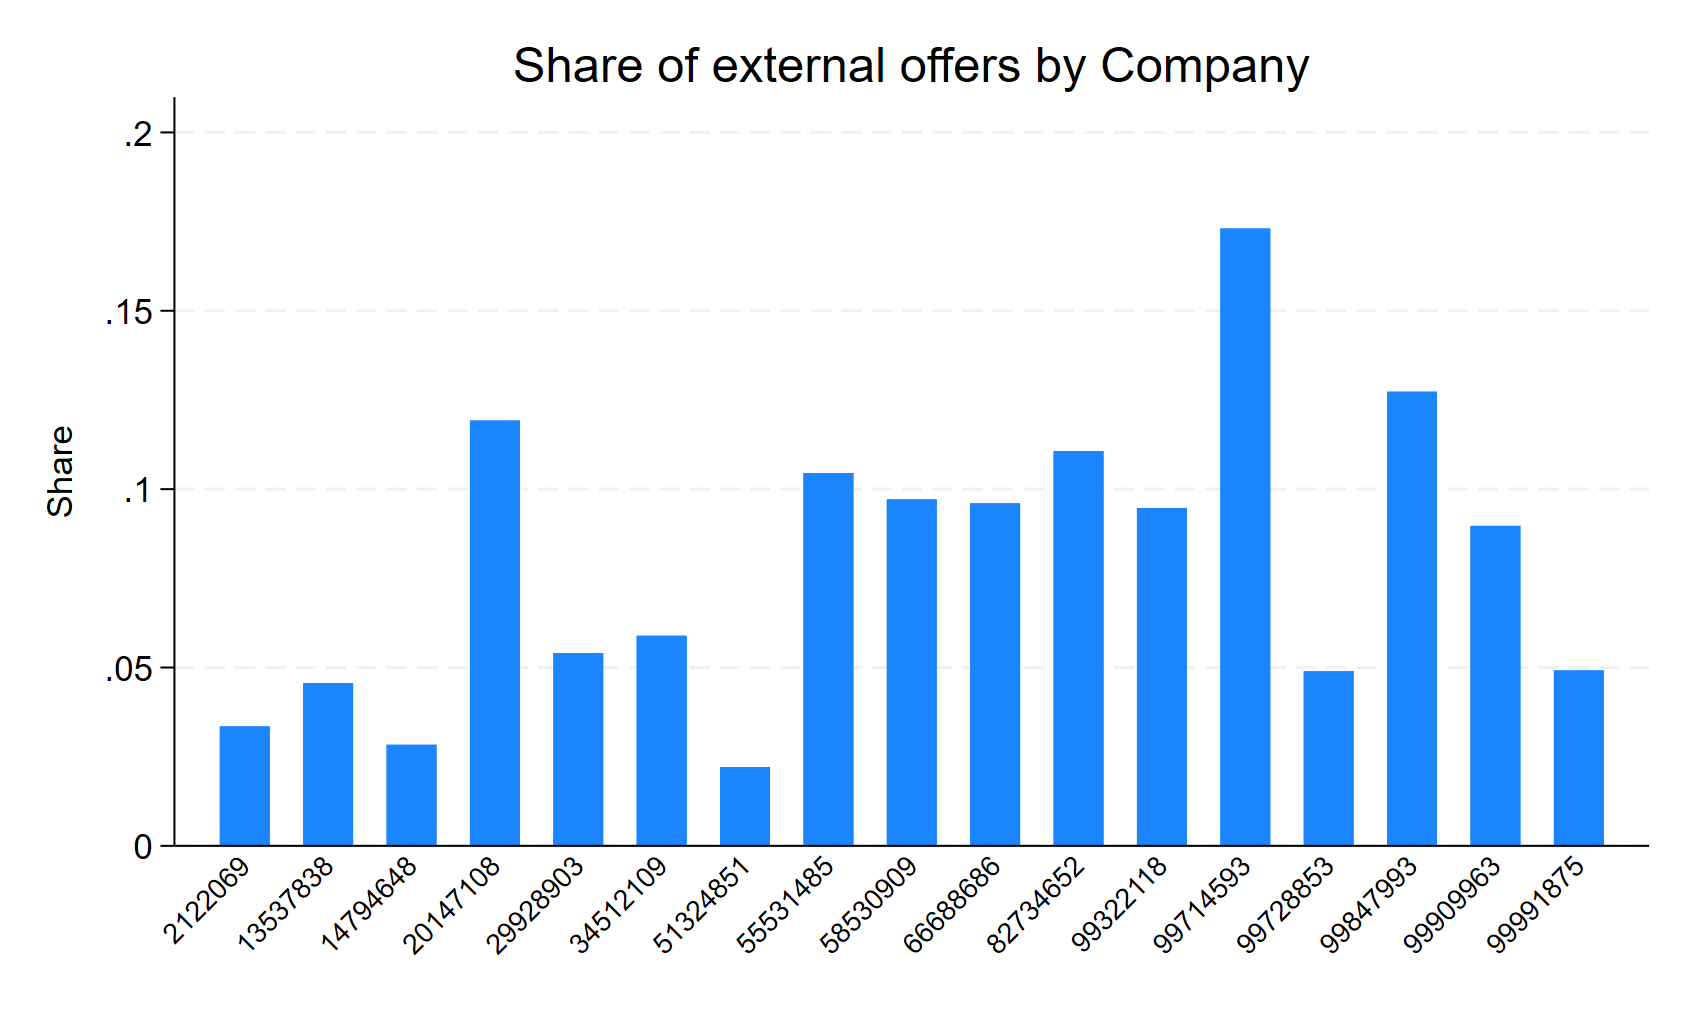
\includegraphics[scale=0.17]{../figures/IE4/IE4_variation_share_external.png}
\end{tabular}
\end{figure} 

\newpage
 
 
\subsection{Negative correlation credit rating and offers}

Offers with better credit ratings make worse offers, this could reflect cost issues or a less elastic demand. 

\begin{figure}[H]
\caption{}
 \label{fig:ie4_4}
\centering{}%
\begin{tabular}{cc}
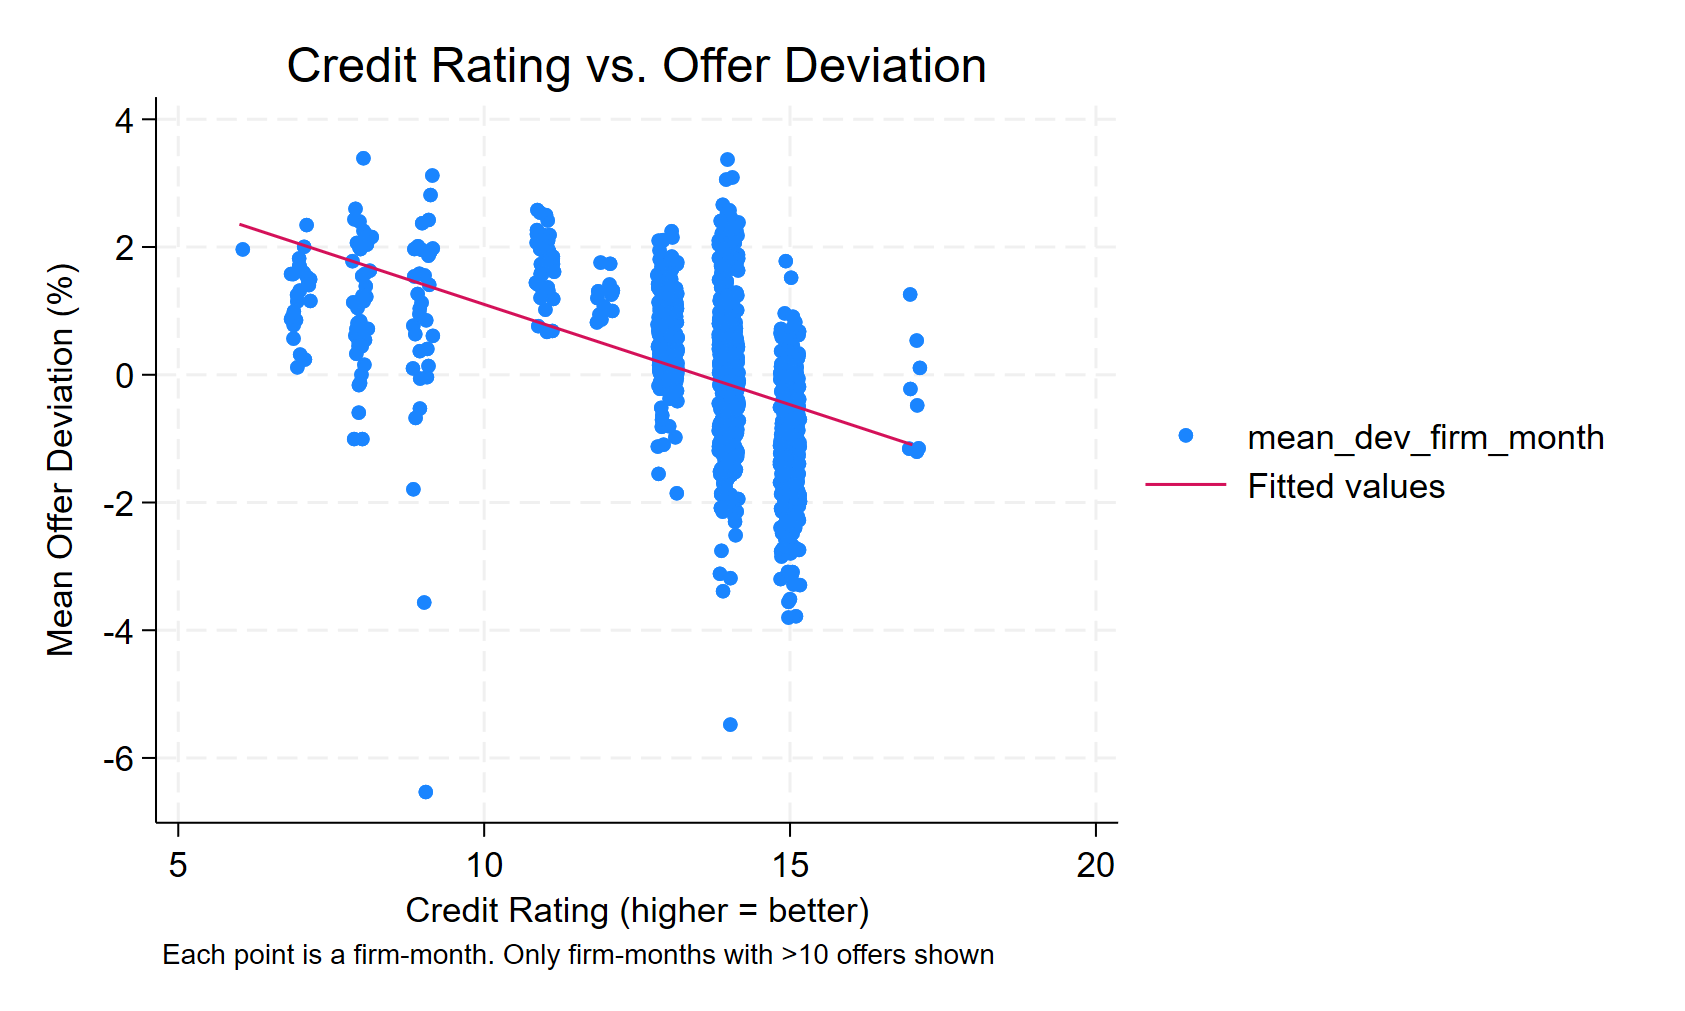
\includegraphics[scale=0.17]{../figures/IE4/IE4_scatter_rating_offer.png} 
\end{tabular}
\end{figure}

\begin{figure}[H]
\caption{}
 \label{fig:ie4_5and6}
\centering{}%
\begin{tabular}{cc}
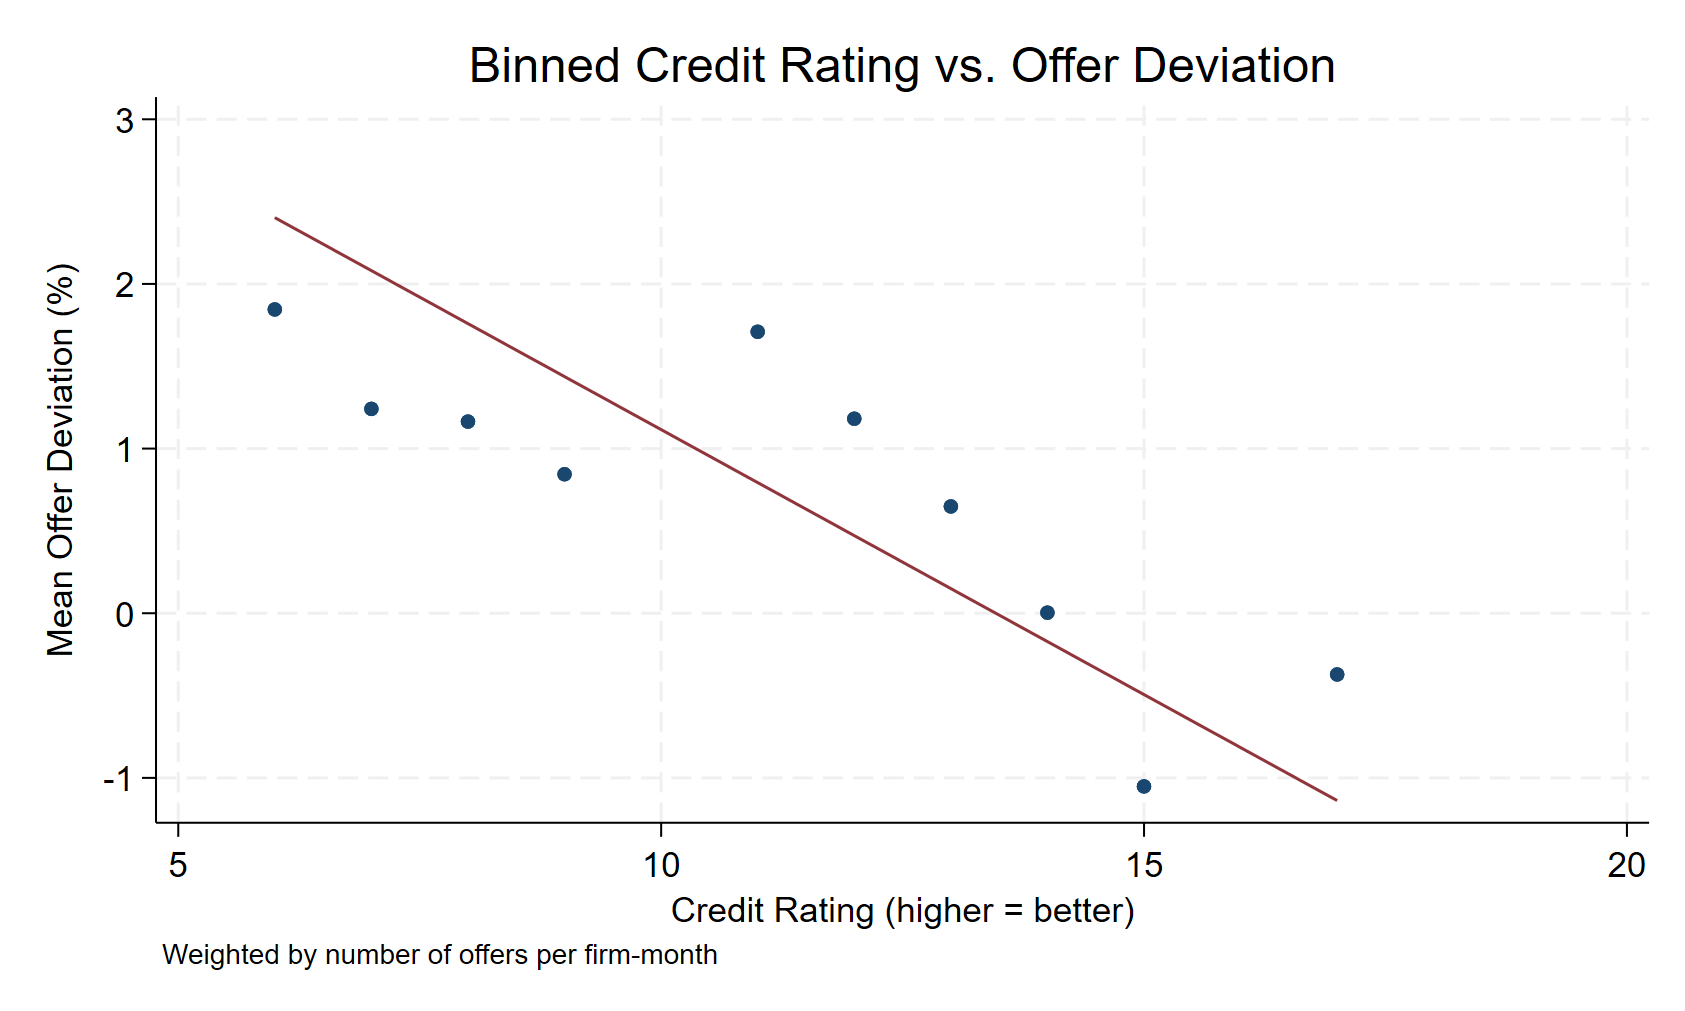
\includegraphics[scale=0.17]{../figures/IE4/IE4_binscatter_rating_offer.png} & 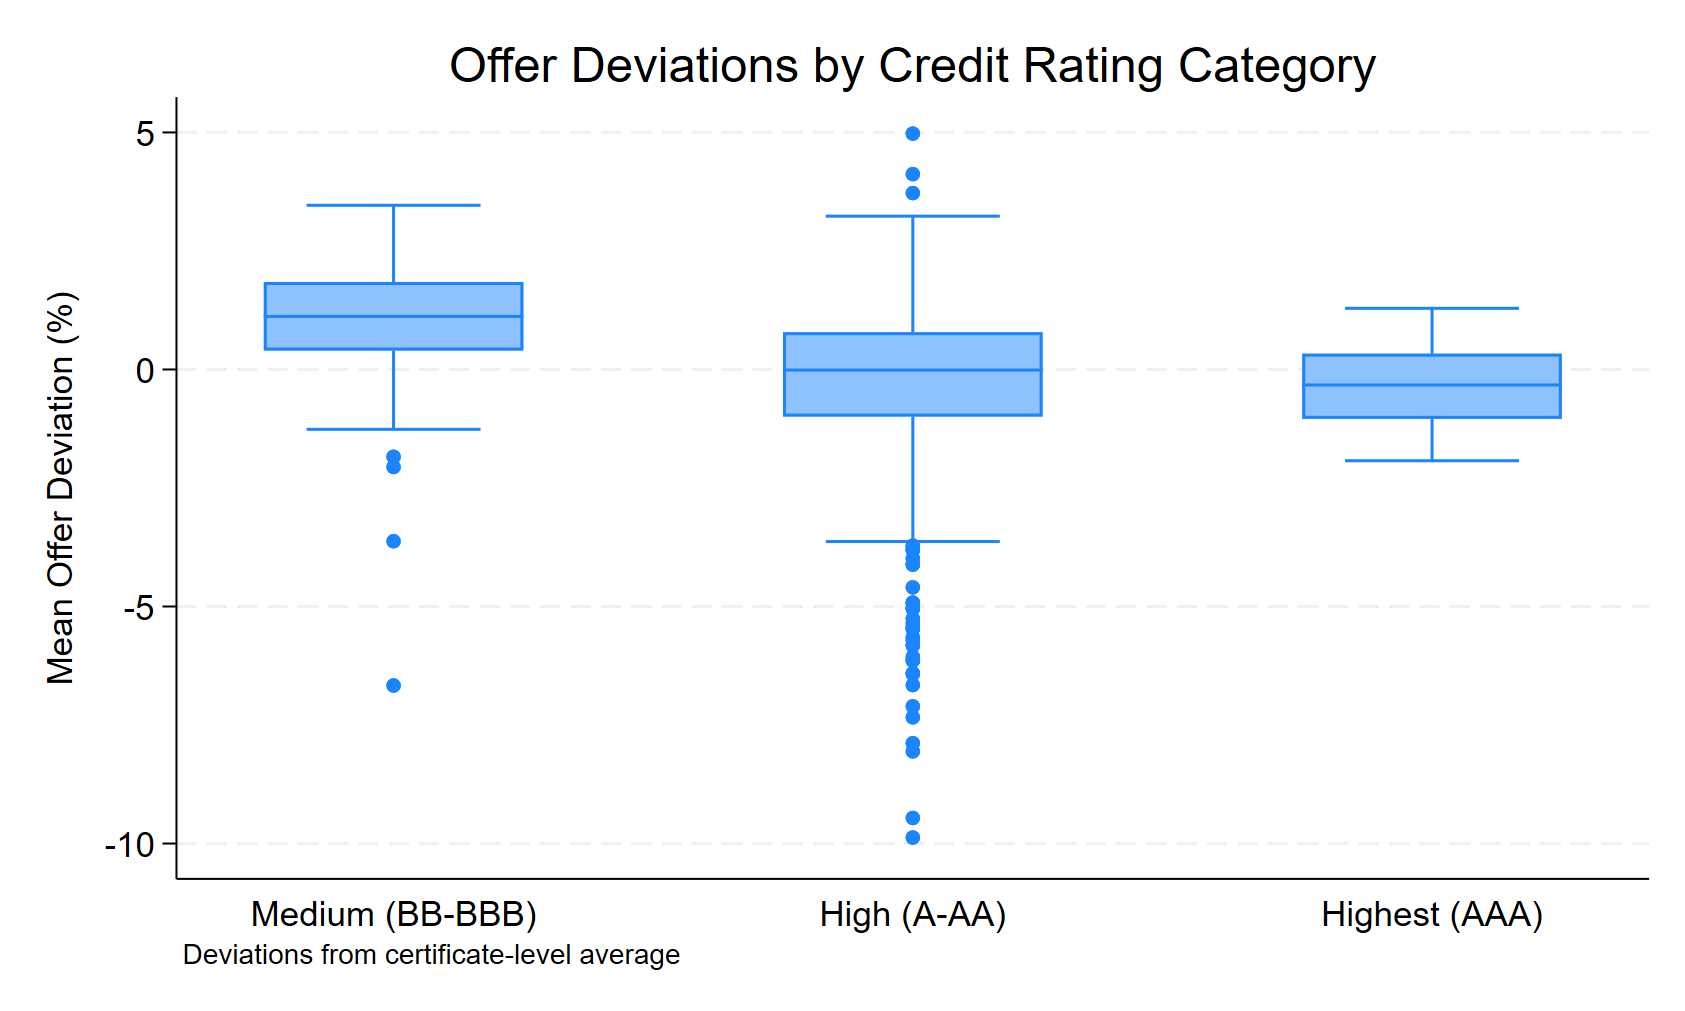
\includegraphics[scale=0.17]{../figures/IE4/IE4_box_rating_offer.png}
\end{tabular}
\end{figure}


Correlation: 
Coefficient: -0.322 (SE:  0.017)



\newpage

\subsection{Intermediaries and external offers}


Figure \ref{fig:ie4_7} shows the distribution of external offers by intermediary use, the table below show the ttest of means, where buyers with intermediaries receive .48 extra external offers, and this number is significant.  
\begin{figure}[H]
\caption{}
 \label{fig:ie4_7}
\centering{}%
\begin{tabular}{cc}
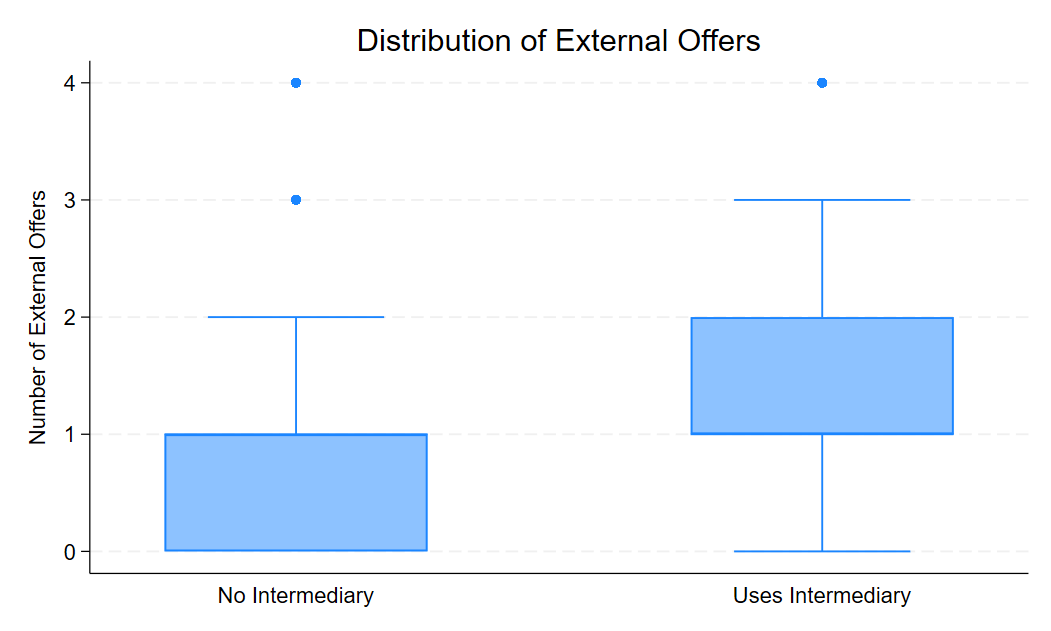
\includegraphics[scale=0.17]{../figures/IE4/IE4_intermediary_search_box.png} 
\end{tabular}
\end{figure}

\begin{table}[htbp]\centering
\def\sym#1{\ifmmode^{#1}\else\(^{#1}\)\fi}
\caption{Search Intensity by Intermediary Use}
\begin{tabular}{l*{1}{ccccc}}
\hline\hline
            &No Intermediary&Has Intermediary&  Difference         & t-statistic&     p-value\\
\hline
n\_ext       &     1.08645&    1.566799&   -.4803491\sym{***}&   -25.95889&    2.3e-146\\
\hline
\(N\)       &       21956&            &                     &            &            \\
\hline\hline
\end{tabular}
\end{table}



 
\newpage

\subsection{Intermediaries and external offers(2)}

Table 3 shows the number of external, initial offers received and  the probability of choosing one of the external offers by intermediary status. Buyers with intermediaries accept external offers at a significantly higher rate than those without them. 

Table 4 shows the number of external offers and the probability of choosing one of the external offers by intermediary type. Buyers with agents receive the least amount of external offers but are the most likely to choose one of them reflecting that they buy from the agent's company. Whereas buyers with advisors receive more offers but are sligthly less likely to buy  from them. Figure \ref{fig:ie4_10} shows similar data and additionally the probability of choosing an external offer having one in the data, which is similar across groups. 
 
\begin{table}[htbp]\centering
\def\sym#1{\ifmmode^{#1}\else\(^{#1}\)\fi}
\caption{Search Behavior by Intermediary Status}
\begin{tabular}{l*{1}{cccc}}
\hline\hline
            &        mean&          sd&         min&       count\\
\hline
0           &            &            &            &            \\
n\_external  &        1.09&        1.33&           0&       10908\\
n\_internal  &       14.09&        7.26&           0&       10908\\
n\_total\_offers&       15.17&        7.75&           1&       10908\\
chose\_external&        0.61&        0.49&           0&       10908\\
\hline
1           &            &            &            &            \\
n\_external  &        1.57&        1.41&           0&       11048\\
n\_internal  &       14.96&        8.81&           0&       11048\\
n\_total\_offers&       16.52&        9.33&           1&       11048\\
chose\_external&        0.91&        0.29&           0&       11048\\
\hline
Total       &            &            &            &            \\
n\_external  &        1.33&        1.39&           0&       21956\\
n\_internal  &       14.52&        8.09&           0&       21956\\
n\_total\_offers&       15.85&        8.61&           1&       21956\\
chose\_external&        0.76&        0.43&           0&       21956\\
\hline
\(N\)       &       21956&            &            &            \\
\hline\hline
\multicolumn{5}{l}{\footnotesize number of searches}\\
\end{tabular}
\end{table}


\begin{table}[htbp]\centering
\def\sym#1{\ifmmode^{#1}\else\(^{#1}\)\fi}
\caption{External Offers by Intermediary Type}
\begin{tabular}{l*{2}{ccc}}
\hline\hline
            &        mean&          sd&       count&        mean&          sd&       count\\
\hline
\hline
\(N\)       &       21956&            &            &       21956&            &            \\
\hline\hline
\end{tabular}
\end{table}


 Figure \ref{fig:ie4_8and9} shows the averaage number of external offers by intermediary tye and the distribution of external offers by having/not having an intermediary. 

 
 
\begin{figure}[H]
\caption{}
 \label{fig:ie4_8and9}
\centering{}%
\begin{tabular}{cc}
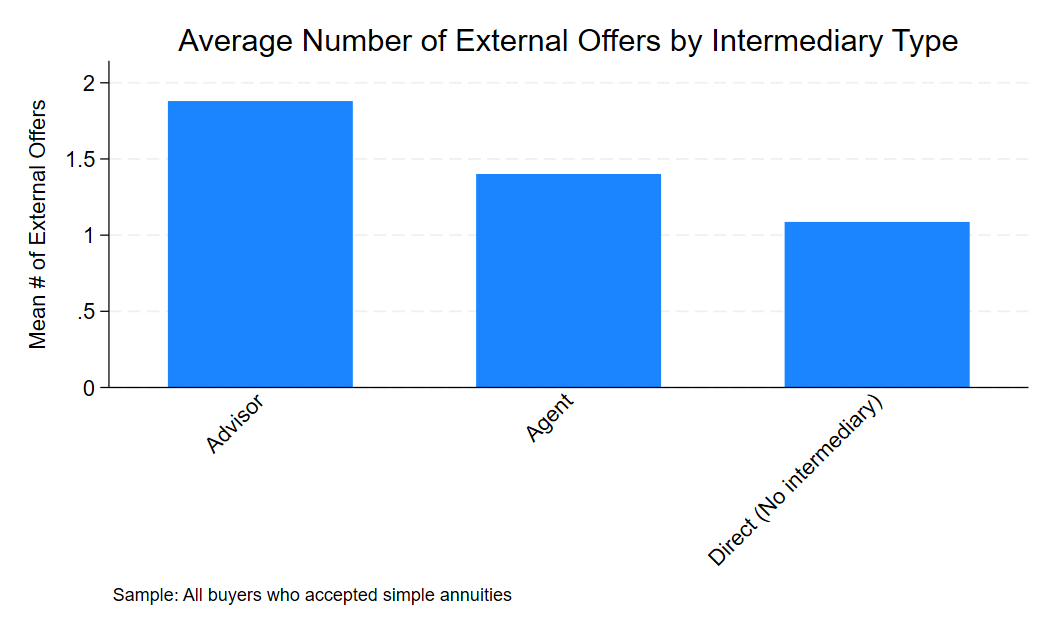
\includegraphics[scale=0.17]{../figures/IE4/IE4_external_offers_by_intermediary.png} & 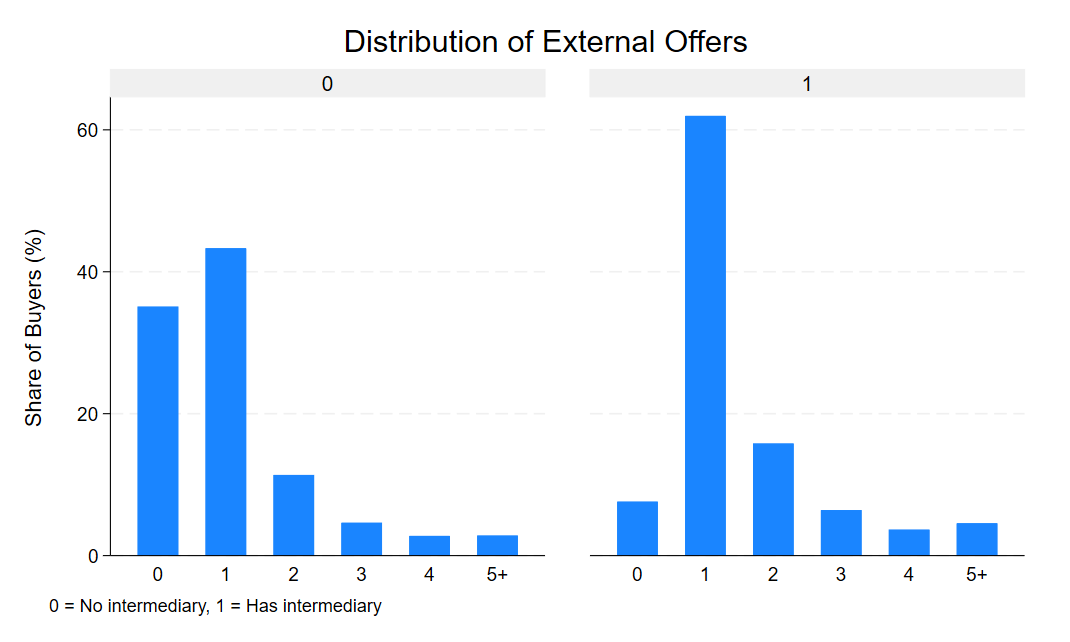
\includegraphics[scale=0.17]{../figures/IE4/IE4_external_distribution_by_intermediary.png} 
\end{tabular}
\end{figure} 
 
\begin{figure}[H]
\caption{}
 \label{fig:ie4_10}
\centering{}%
\begin{tabular}{cc}
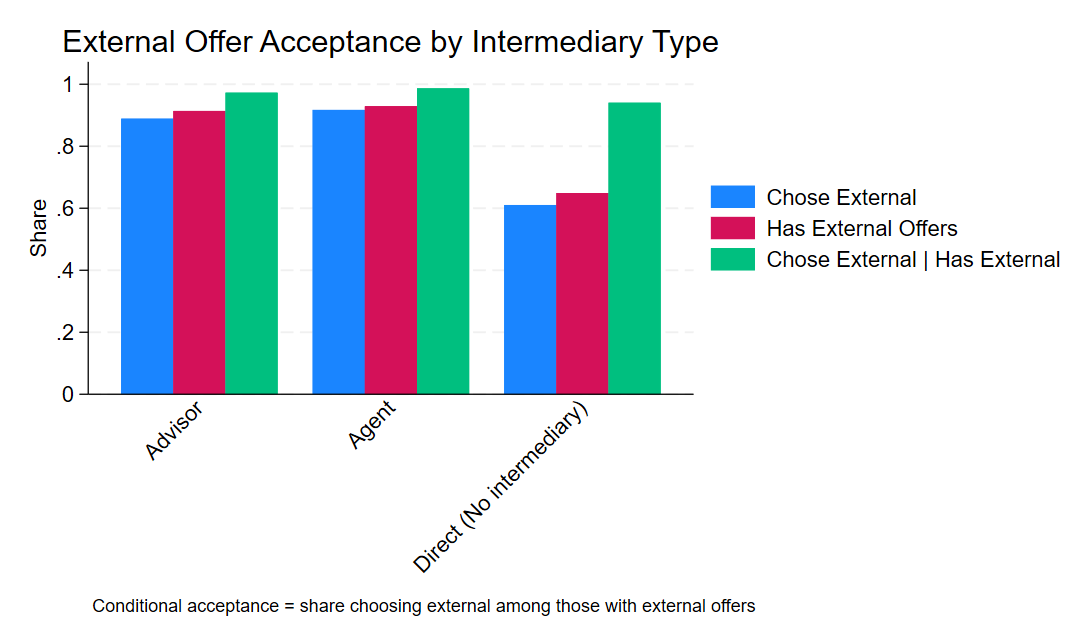
\includegraphics[scale=0.17]{../figures/IE4/IE4_external_acceptance_by_intermediary.png} 
\end{tabular}
\end{figure} 
 
Table 5 shows that intermediariees generally increase the number of external offers, but when desaggregating the effect, agents actually generate less offers and brokers are the ones driving the increase in offers. 
 \input{../Tables/ie4/ie4_regression_external.tex}

 Table 6, shows that intermediareis increase the chances of accepting an external offer,  conditionaal on having offers, but this is driven mainly by agents and not by brokers.

  \begin{table}[htbp]\centering
\def\sym#1{\ifmmode^{#1}\else\(^{#1}\)\fi}
\caption{Probability of Choosing External Offer (Conditional on Having External)}
\begin{tabular}{l*{2}{c}}
\hline\hline
                    &\multicolumn{1}{c}{(1)}         &\multicolumn{1}{c}{(2)}         \\
\hline
chose\_external      &                     &                     \\
has\_intermediary    &       1.245\sym{***}&                     \\
                    &     (0.090)         &                     \\
[1em]
A                   &                     &       0.000         \\
                    &                     &         (.)         \\
[1em]
D                   &                     &      -1.562\sym{***}\\
                    &                     &     (0.118)         \\
[1em]
P                   &                     &      -0.742\sym{***}\\
                    &                     &     (0.149)         \\
[1em]
Constant            &       2.759\sym{***}&       4.321\sym{***}\\
                    &     (0.050)         &     (0.107)         \\
\hline
Obs.                &      17,289         &      17,289         \\
\hline\hline
\end{tabular}
\end{table}

figure \ref{fig:ie4_11} shows that buyers with intermediaries receive more offers along the income distribution. 
  \begin{figure}[H]
\caption{}
 \label{fig:ie4_11}
\centering{}%
\begin{tabular}{cc}
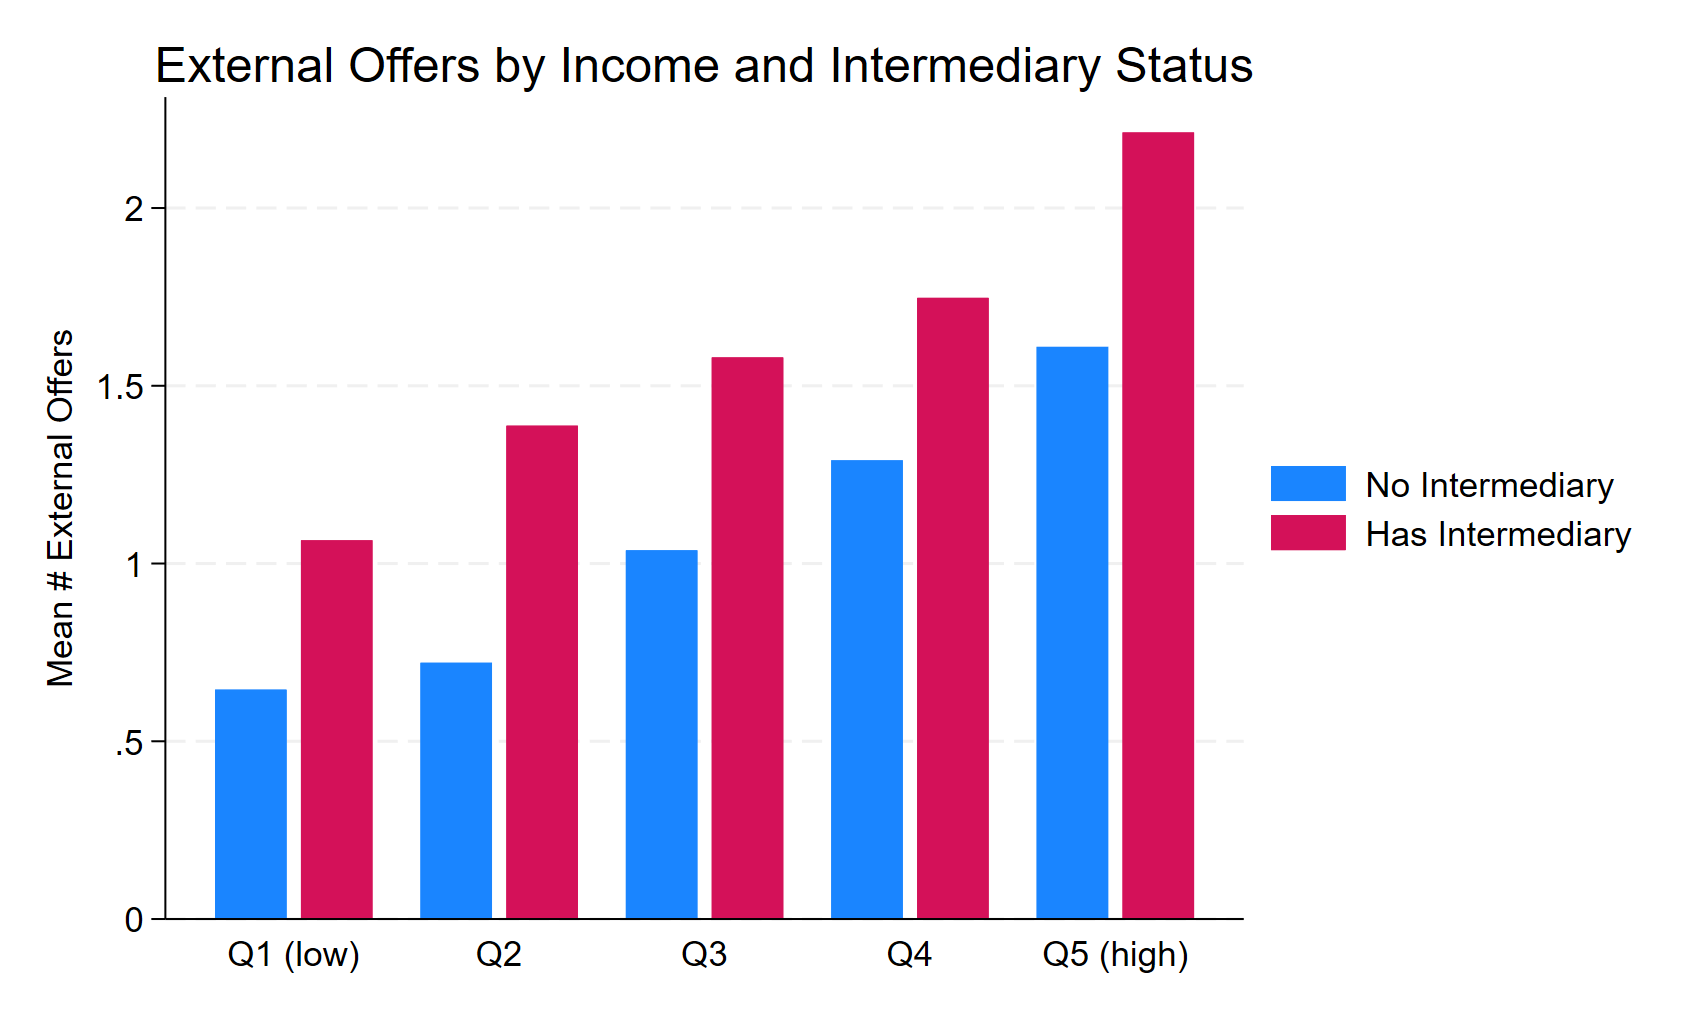
\includegraphics[scale=0.27]{../figures/IE4/IE4_external_by_income_intermediary.png} 
\end{tabular}
\end{figure} 

\newpage

 
\subsection{Choose highest offer and Intermediaries}

Table 7 shows the share of buyers choosing the highest income, the foregone percentage in case (difference between highest and chosen offer) and the total number of offers by income quintile. Richer individuals receive higher offers but there is no clear pattern in the share of buyers choosing the highest offer or in the foregone percentage over income quintiles. Figure \ref{fig:ie4_12} shows the sam pattern of the share of buyers choosing the highest offer by income quintile. 


\begin{table}[htbp]\centering
\def\sym#1{\ifmmode^{#1}\else\(^{#1}\)\fi}
\caption{Choosing Highest Offer by Income Quintile}
\begin{tabular}{l*{1}{ccc}}
\hline\hline
            &        mean&          sd&       count\\
\hline
Q1(low)     &            &            &            \\
chose\_highest\_cert&       0.516&       0.500&        3700\\
foregone\_pct&       1.076&       1.585&        3700\\
foregone\_pct2&       2.222&       1.626&        1791\\
n\_total\_offers&       7.571&       4.231&        3700\\
\hline
Q2          &            &            &            \\
chose\_highest\_cert&       0.550&       0.498&        3659\\
foregone\_pct&       0.674&       1.094&        3659\\
foregone\_pct2&       1.497&       1.195&        1648\\
n\_total\_offers&      12.286&       4.705&        3659\\
\hline
Q3          &            &            &            \\
chose\_highest\_cert&       0.574&       0.495&        3644\\
foregone\_pct&       0.568&       0.999&        3644\\
foregone\_pct2&       1.332&       1.151&        1554\\
n\_total\_offers&      15.037&       5.649&        3644\\
\hline
Q4          &            &            &            \\
chose\_highest\_cert&       0.576&       0.494&        3640\\
foregone\_pct&       0.594&       1.121&        3640\\
foregone\_pct2&       1.402&       1.355&        1542\\
n\_total\_offers&      17.129&       6.833&        3640\\
\hline
Q5(high)    &            &            &            \\
chose\_highest\_cert&       0.505&       0.500&        3649\\
foregone\_pct&       0.782&       1.348&        3649\\
foregone\_pct2&       1.579&       1.553&        1807\\
n\_total\_offers&      17.362&       7.377&        3649\\
\hline
Total       &            &            &            \\
chose\_highest\_cert&       0.544&       0.498&       18292\\
foregone\_pct&       0.740&       1.262&       18292\\
foregone\_pct2&       1.622&       1.436&        8342\\
n\_total\_offers&      13.857&       6.920&       18292\\
\hline
\(N\)       &       18292&            &            \\
\hline\hline
\end{tabular}
\end{table}


  \begin{figure}[H]
\caption{}
 \label{fig:ie4_12}
\centering{}%
\begin{tabular}{cc}
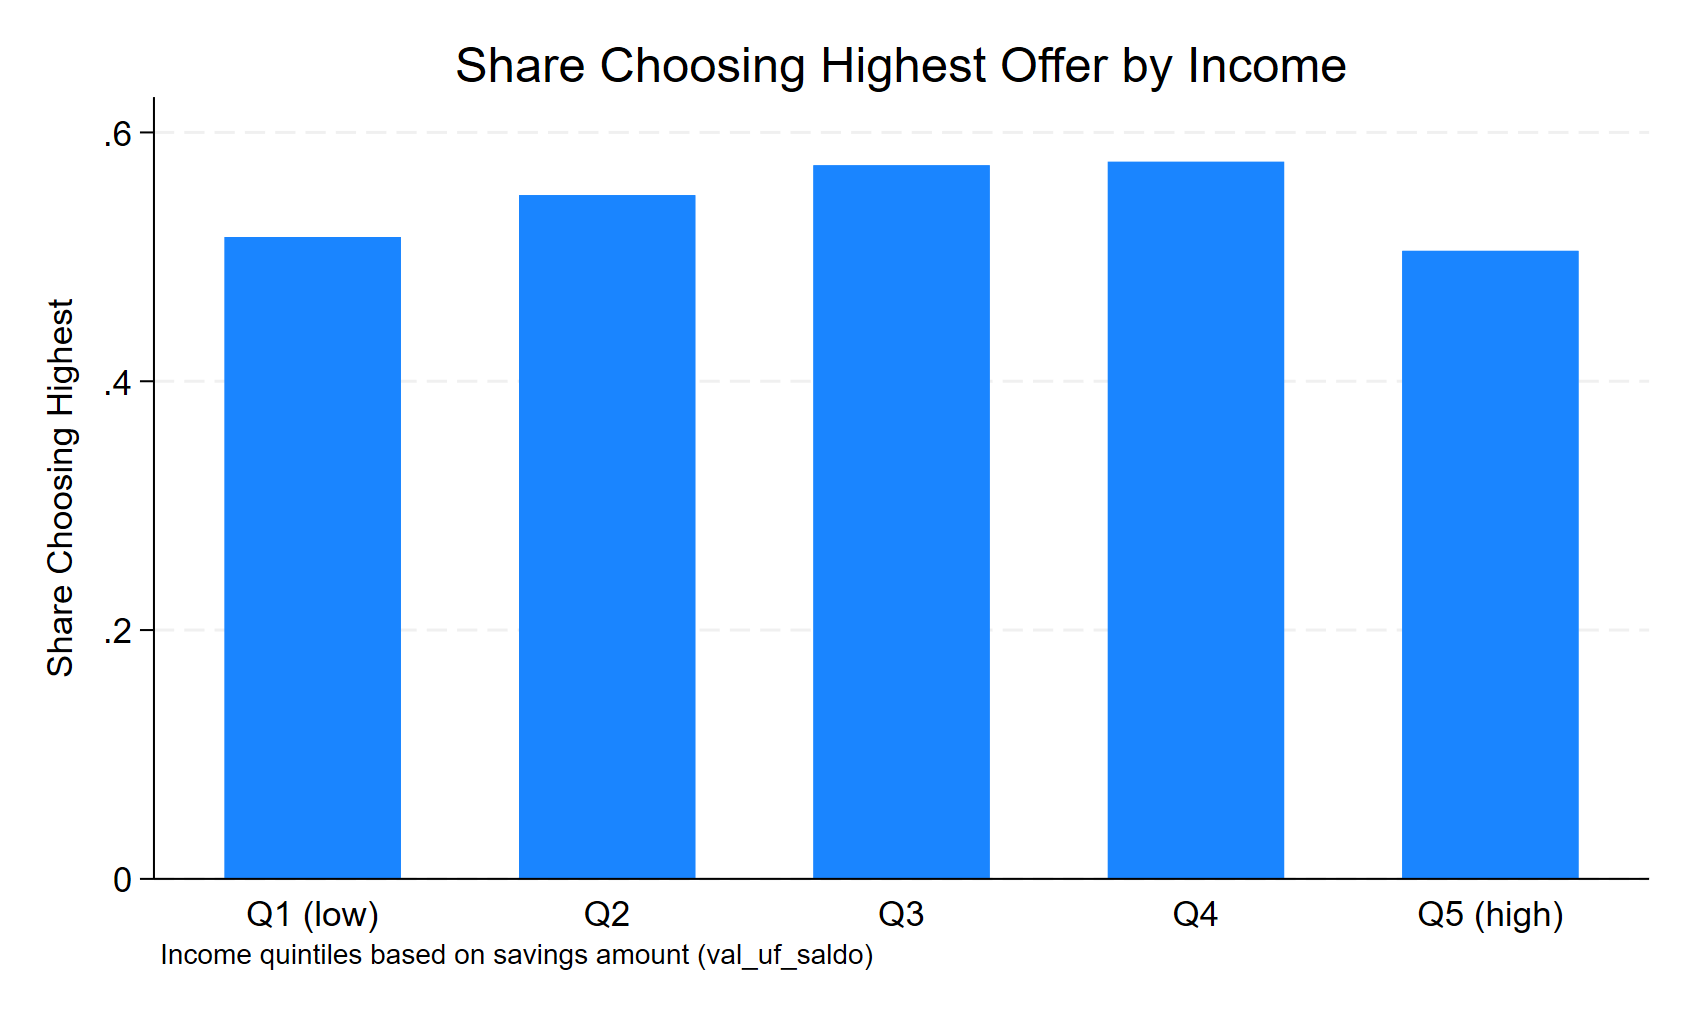
\includegraphics[scale=0.27]{../figures/IE4/IE4_highest_by_income.png} 
\end{tabular}
\end{figure} 

Table 8 shows that buyers with intermediaries have a lower likelihood of choosing the highest offer (first row in each subtable) and when they choose lower offers they forego a higher percentage of income (third row of each subtable).
Figure \ref{fig:ie4_11} shows that actually this effect of intermediaries is driven by sales agents, and buyers with brokers actually choose the highest offer at a higher rate that those without any intermediaries. 

\begin{table}[htbp]\centering
\def\sym#1{\ifmmode^{#1}\else\(^{#1}\)\fi}
\caption{Choosing Highest Offer by Intermediary Status}
\begin{tabular}{l*{1}{ccc}}
\hline\hline
            &        mean&          sd&       count\\
\hline
0           &            &            &            \\
chose\_highest\_cert&       0.629&       0.483&        9507\\
foregone\_pct&       0.518&       1.047&        9507\\
foregone\_pct2&       1.398&       1.315&        3524\\
n\_total\_offers&      13.501&       6.185&        9507\\
\hline
1           &            &            &            \\
chose\_highest\_cert&       0.452&       0.498&        8785\\
foregone\_pct&       0.979&       1.421&        8785\\
foregone\_pct2&       1.786&       1.498&        4818\\
n\_total\_offers&      14.242&       7.618&        8785\\
\hline
Total       &            &            &            \\
chose\_highest\_cert&       0.544&       0.498&       18292\\
foregone\_pct&       0.740&       1.262&       18292\\
foregone\_pct2&       1.622&       1.436&        8342\\
n\_total\_offers&      13.857&       6.920&       18292\\
\hline
\(N\)       &       18292&            &            \\
\hline\hline
\end{tabular}
\end{table}



 
\begin{figure}[H]
\caption{}
 \label{fig:ie4_11}
\centering{}%
\begin{tabular}{cc}
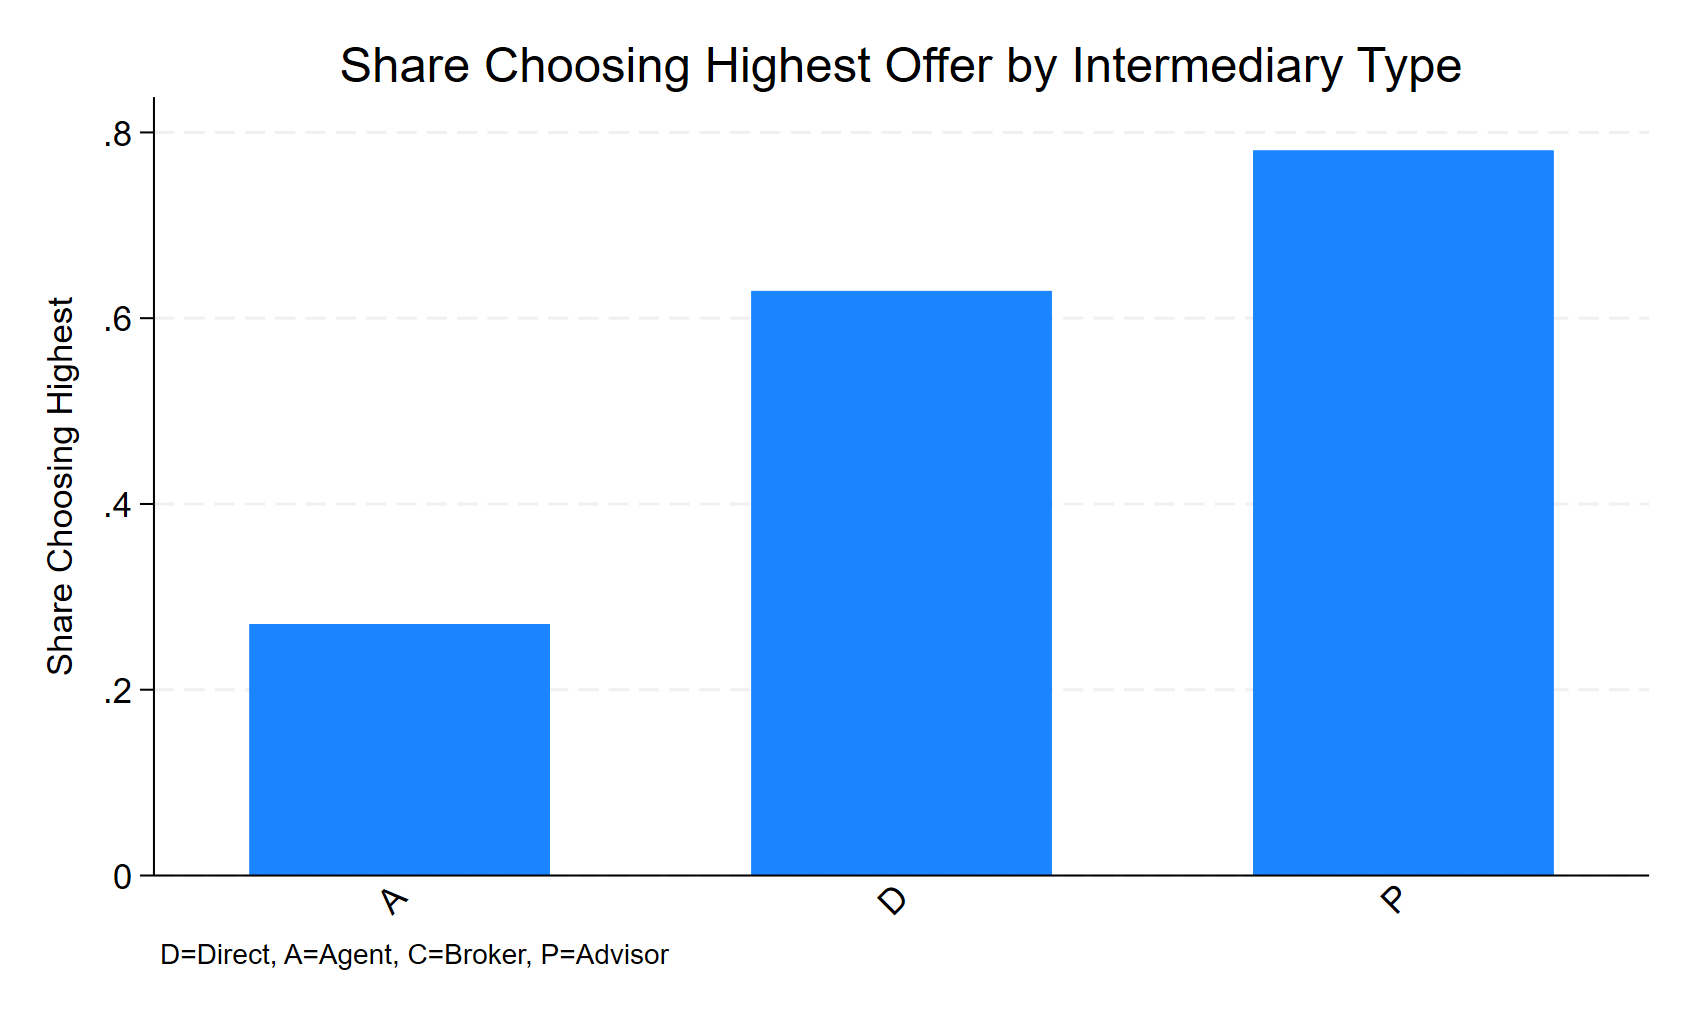
\includegraphics[scale=0.17]{../figures/IE4/IE4_highest_by_intermediary_type.png} 
& 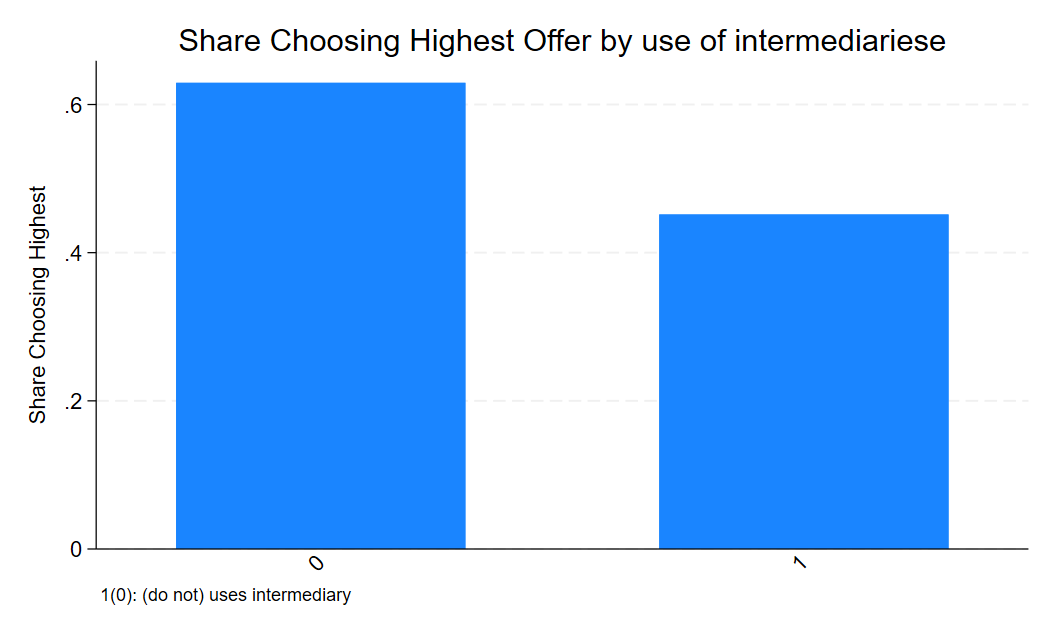
\includegraphics[scale=0.17]{../figures/IE4/IE4_highest_by_intermediary_type(2).png} 
\end{tabular}
\end{figure} 
 
Table 9 shos the patterns of table 8 but for buyers with and without external offers. Both types of buyers have a similar rate at which they choose the lower offers, this is not consistent with the idea that external offers are requested from firms with particularly good non-offer characteristics. 

\begin{table}[htbp]\centering
\def\sym#1{\ifmmode^{#1}\else\(^{#1}\)\fi}
\caption{Choosing Highest Offer by External Offer Status}
\begin{tabular}{l*{6}{ccc}}
\hline\hline
            &        mean&          sd&       count&        mean&          sd&       count&        mean&          sd&       count&        mean&          sd&       count&        mean&          sd&       count&        mean&          sd&       count\\
\hline
\hline
\(N\)       &       18292&            &            &       18292&            &            &       18292&            &            &       18292&            &            &       18292&            &            &        8342&            &            \\
\hline\hline
\end{tabular}
\end{table}


Finally figures \ref{fig:ie4_12and13} show the patterns of the share of buyers choosing the highest offer by income quintile for buyers with and without intermediaries and with and without external offers.
  \begin{figure}[H]
\caption{}
 \label{fig:ie4_12and13}
\centering{}%
\begin{tabular}{cc}
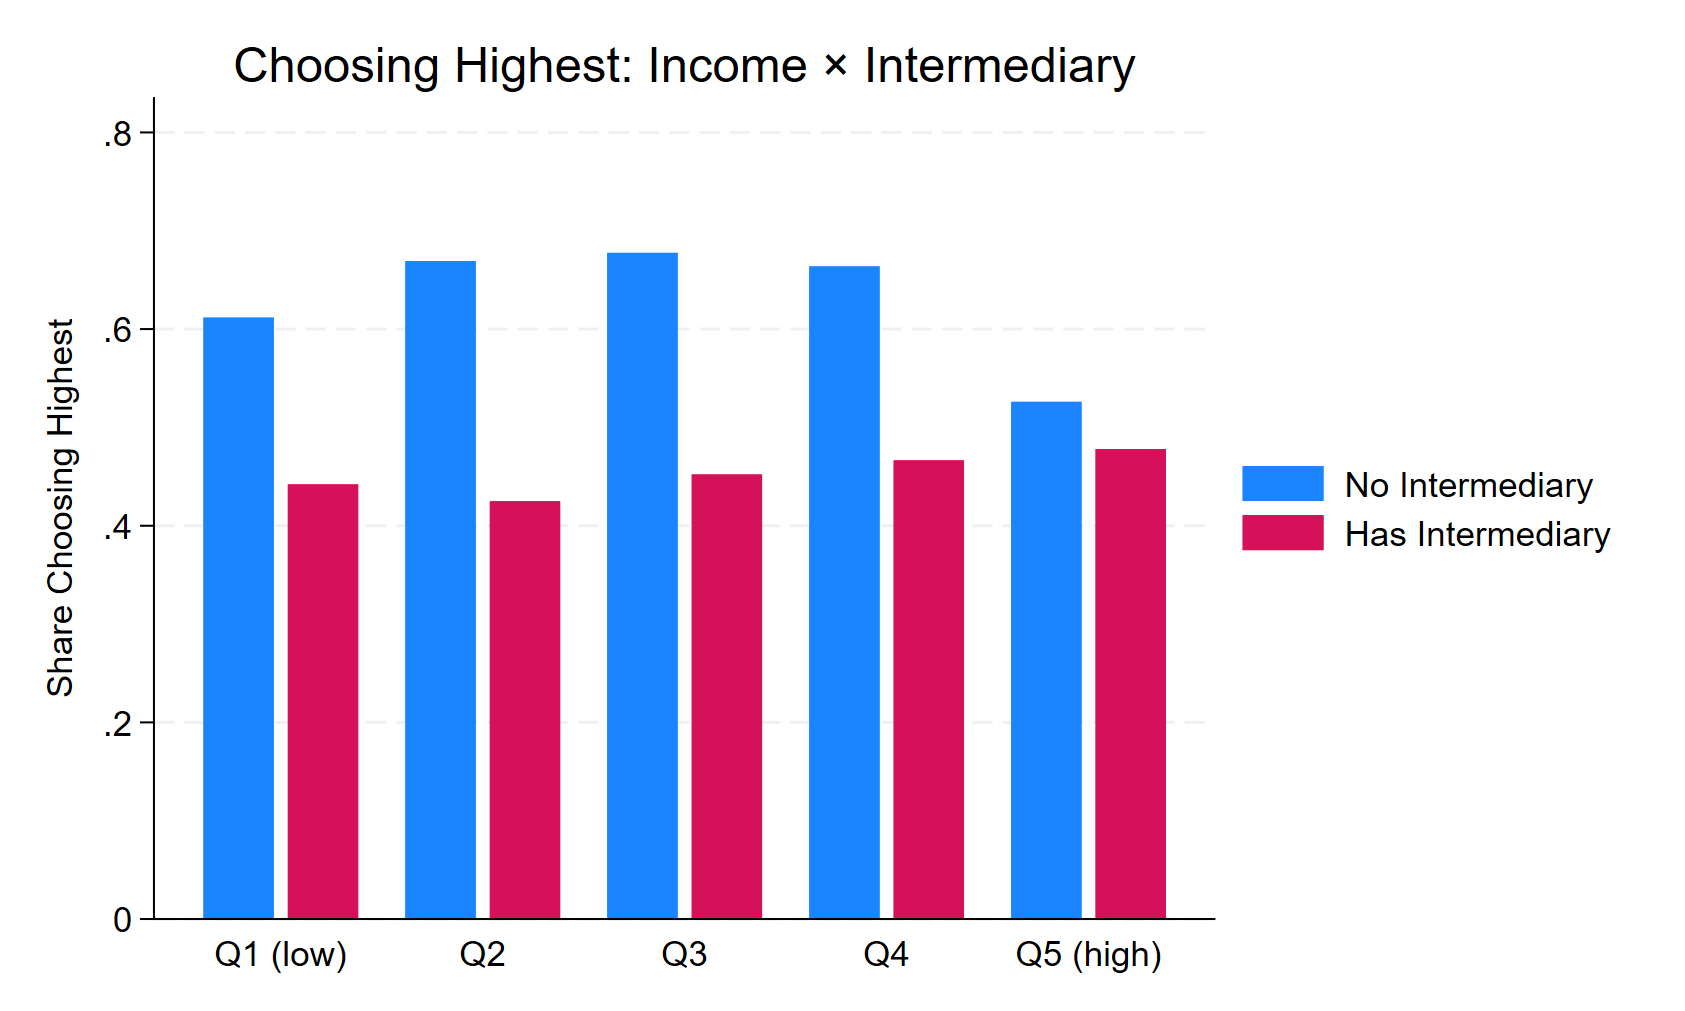
\includegraphics[scale=0.17]{../figures/IE4/IE4_highest_income_intermediary.png} & 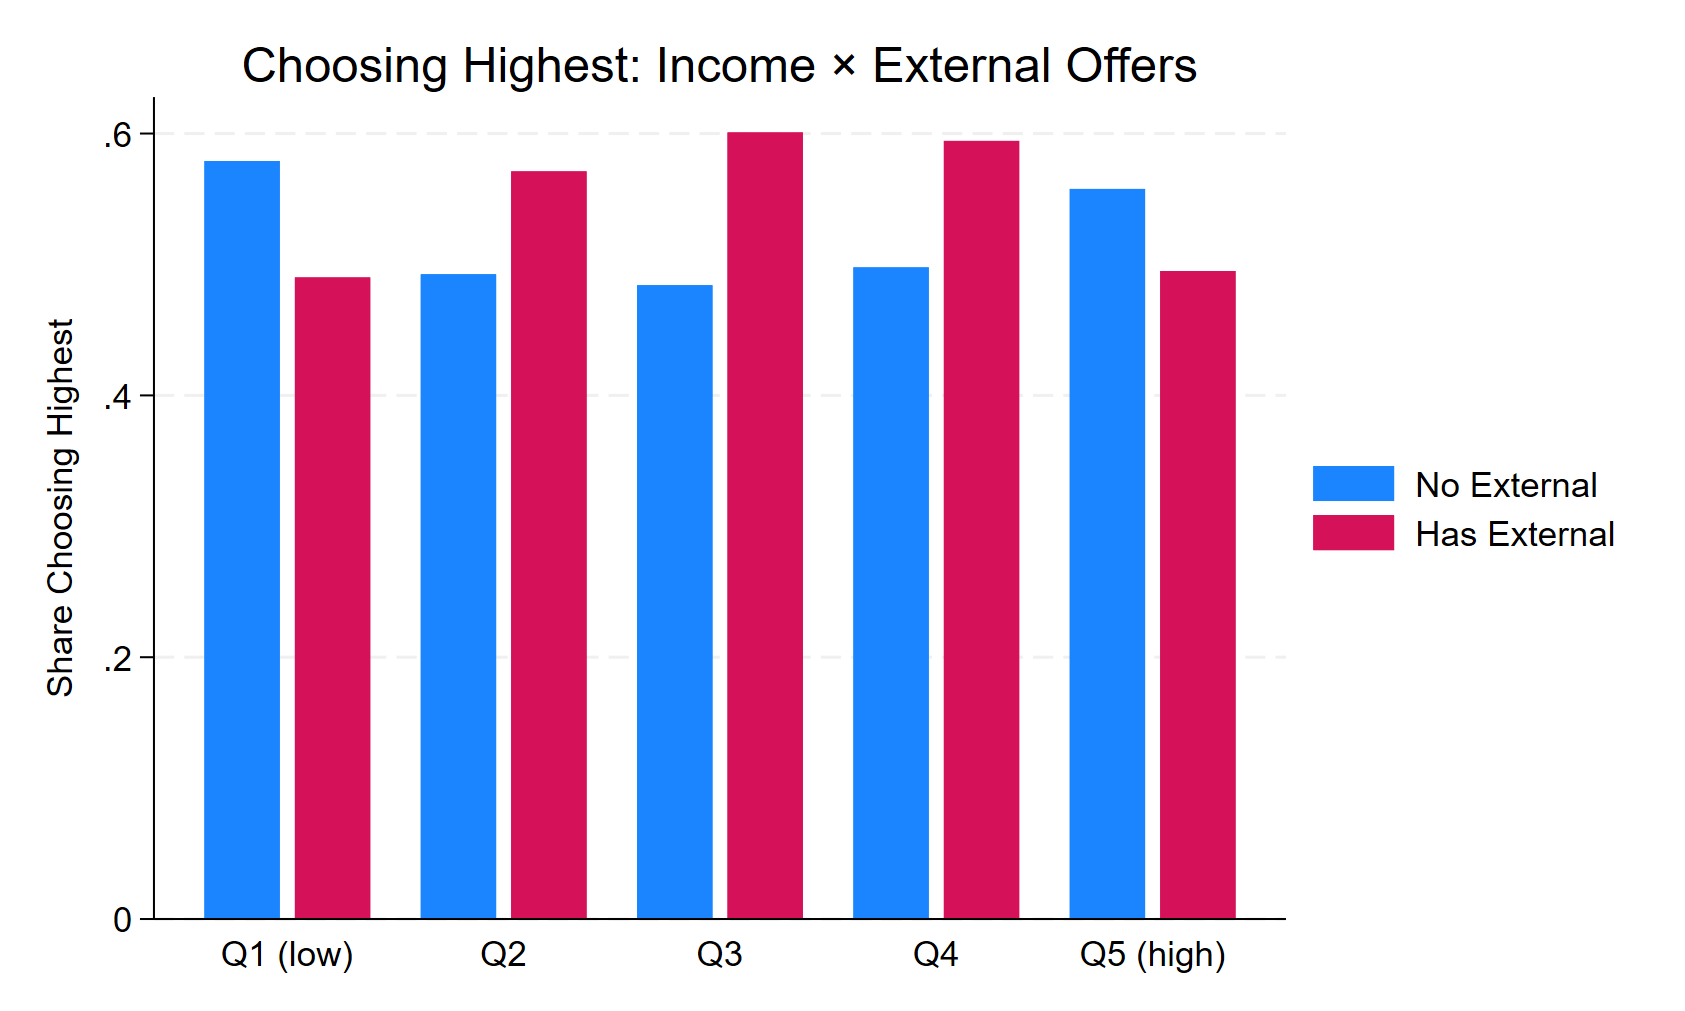
\includegraphics[scale=0.17]{../figures/IE4/IE4_highest_income_external.png} 
\end{tabular}
\end{figure} 


\begin{table}[htbp]\centering
\def\sym#1{\ifmmode^{#1}\else\(^{#1}\)\fi}
\caption{Determinants of Choosing Highest Offer}
\begin{tabular}{l*{5}{c}}
\hline\hline
            &\multicolumn{1}{c}{(1)}         &\multicolumn{1}{c}{(2)}         &\multicolumn{1}{c}{(3)}         &\multicolumn{1}{c}{(4)}         &\multicolumn{1}{c}{(5)}         \\
\hline
main        &                     &                     &                     &                     &                     \\
has\_intermediary&      -0.867\sym{***}&      -0.879\sym{***}&      -0.873\sym{***}&                     &      -0.209\sym{***}\\
            &     (0.033)         &     (0.033)         &     (0.033)         &                     &     (0.008)         \\
[1em]
has\_external&       0.475\sym{***}&       0.498\sym{***}&       0.418\sym{***}&                     &       0.098\sym{***}\\
            &     (0.040)         &     (0.040)         &     (0.046)         &                     &     (0.011)         \\
[1em]
1.income\_q  &                     &       0.000         &       0.000         &       0.000         &       0.000         \\
            &                     &         (.)         &         (.)         &         (.)         &         (.)         \\
[1em]
2.income\_q  &                     &       0.066         &       0.207\sym{***}&       0.211\sym{***}&       0.049\sym{***}\\
            &                     &     (0.048)         &     (0.049)         &     (0.049)         &     (0.012)         \\
[1em]
3.income\_q  &                     &       0.122\sym{**} &       0.337\sym{***}&       0.335\sym{***}&       0.079\sym{***}\\
            &                     &     (0.048)         &     (0.052)         &     (0.052)         &     (0.012)         \\
[1em]
4.income\_q  &                     &       0.095\sym{*}  &       0.360\sym{***}&       0.351\sym{***}&       0.085\sym{***}\\
            &                     &     (0.048)         &     (0.055)         &     (0.055)         &     (0.013)         \\
[1em]
5.income\_q  &                     &      -0.222\sym{***}&       0.009         &       0.026         &       0.003         \\
            &                     &     (0.049)         &     (0.056)         &     (0.056)         &     (0.013)         \\
[1em]
n\_total\_offers&                     &                     &      -0.033\sym{***}&      -0.025\sym{***}&      -0.008\sym{***}\\
            &                     &                     &     (0.003)         &     (0.003)         &     (0.001)         \\
[1em]
n\_external  &                     &                     &       0.112\sym{***}&                     &       0.026\sym{***}\\
            &                     &                     &     (0.017)         &                     &     (0.004)         \\
[1em]
0.has\_intermediary&                     &                     &                     &       0.000         &                     \\
            &                     &                     &                     &         (.)         &                     \\
[1em]
1.has\_intermediary&                     &                     &                     &       0.028         &                     \\
            &                     &                     &                     &     (0.083)         &                     \\
[1em]
0.has\_external&                     &                     &                     &       0.000         &                     \\
            &                     &                     &                     &         (.)         &                     \\
[1em]
1.has\_external&                     &                     &                     &       0.809\sym{***}&                     \\
            &                     &                     &                     &     (0.045)         &                     \\
[1em]
0.has\_intermediary#0.has\_external&                     &                     &                     &       0.000         &                     \\
            &                     &                     &                     &         (.)         &                     \\
[1em]
0.has\_intermediary#1.has\_external&                     &                     &                     &       0.000         &                     \\
            &                     &                     &                     &         (.)         &                     \\
[1em]
1.has\_intermediary#0.has\_external&                     &                     &                     &       0.000         &                     \\
            &                     &                     &                     &         (.)         &                     \\
[1em]
1.has\_intermediary#1.has\_external&                     &                     &                     &      -1.056\sym{***}&                     \\
            &                     &                     &                     &     (0.090)         &                     \\
[1em]
\_cons      &       0.235\sym{***}&       0.211\sym{***}&       0.416\sym{***}&       0.181\sym{***}&       0.600\sym{***}\\
            &     (0.032)         &     (0.044)         &     (0.047)         &     (0.048)         &     (0.011)         \\
\hline
Obs.        &      18,292         &      18,292         &      18,292         &      18,292         &      18,292         \\
Pseudo R2   &       0.029         &       0.032         &       0.038         &       0.041         &                     \\
\hline\hline
\multicolumn{6}{l}{\footnotesize Models 1-4: Logit. Model 5: LPM. Robust standard errors.}\\
\end{tabular}
\end{table}




  \begin{figure}[H]
\caption{}
 \label{fig:ie4_11}
\centering{}%
\begin{tabular}{cc}
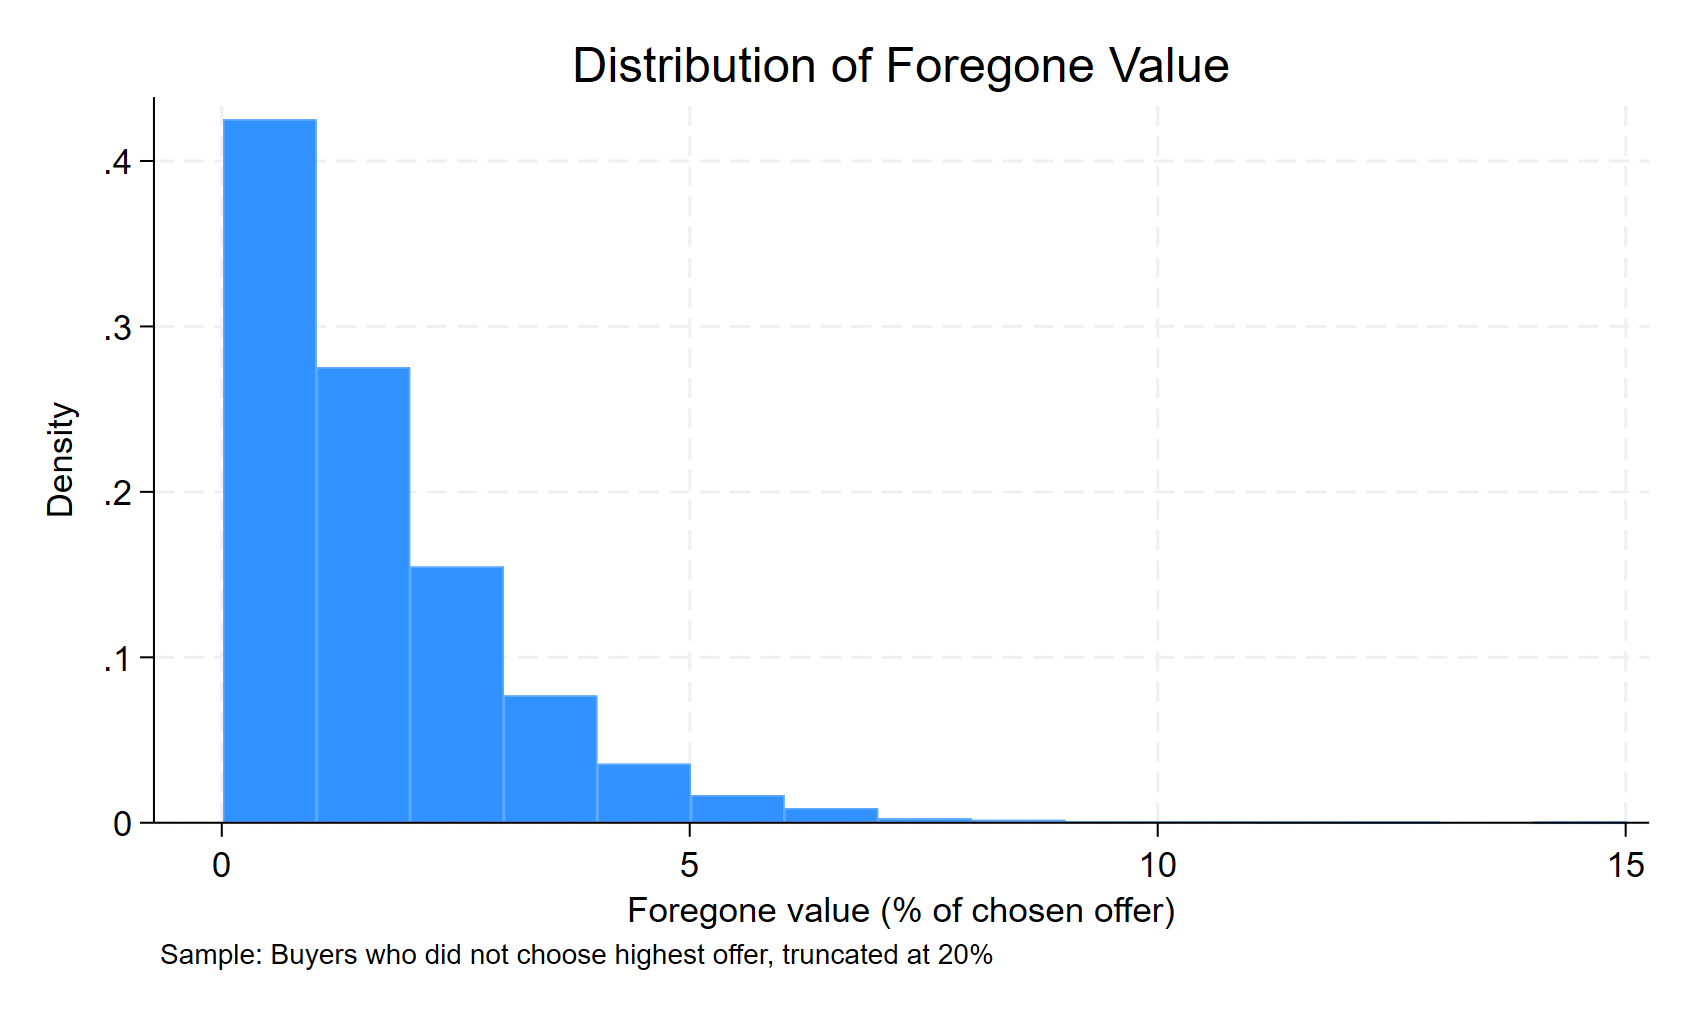
\includegraphics[scale=0.27]{../figures/IE4/IE4_foregone_distribution.png} 
\end{tabular}
\end{figure} 


\begin{table}[htbp]\centering
\def\sym#1{\ifmmode^{#1}\else\(^{#1}\)\fi}
\caption{Determinants of Foregone Value}
\begin{tabular}{l*{1}{c}}
\hline\hline
            &\multicolumn{1}{c}{(1)}         \\
\hline
has\_intermediary&       0.498\sym{***}\\
            &     (0.034)         \\
[1em]
has\_external&      -0.287\sym{***}\\
            &     (0.041)         \\
[1em]
1.income\_q  &       0.000         \\
            &         (.)         \\
[1em]
2.income\_q  &      -0.680\sym{***}\\
            &     (0.048)         \\
[1em]
3.income\_q  &      -0.791\sym{***}\\
            &     (0.049)         \\
[1em]
4.income\_q  &      -0.660\sym{***}\\
            &     (0.055)         \\
[1em]
5.income\_q  &      -0.408\sym{***}\\
            &     (0.059)         \\
[1em]
n\_total\_offers&      -0.012\sym{***}\\
            &     (0.002)         \\
[1em]
\_cons      &       2.217\sym{***}\\
            &     (0.050)         \\
\hline
Obs.        &       8,342         \\
R-squared   &       0.075         \\
\hline\hline
\multicolumn{2}{l}{\footnotesize Sample: Buyers who did not choose highest offer. DV: Foregone }\\
\end{tabular}
\end{table}



\newpage

\subsection{External offer ranking when accepted}

External offers are different (\ref{fig:ie4_11}), the difference is significant, see wilcoxon rank-sum. Table 12 shows a similar pattern. 
\begin{figure}[H]
\caption{}
\label{fig:ie4_11}
\centering{}%
\begin{tabular}{cc}
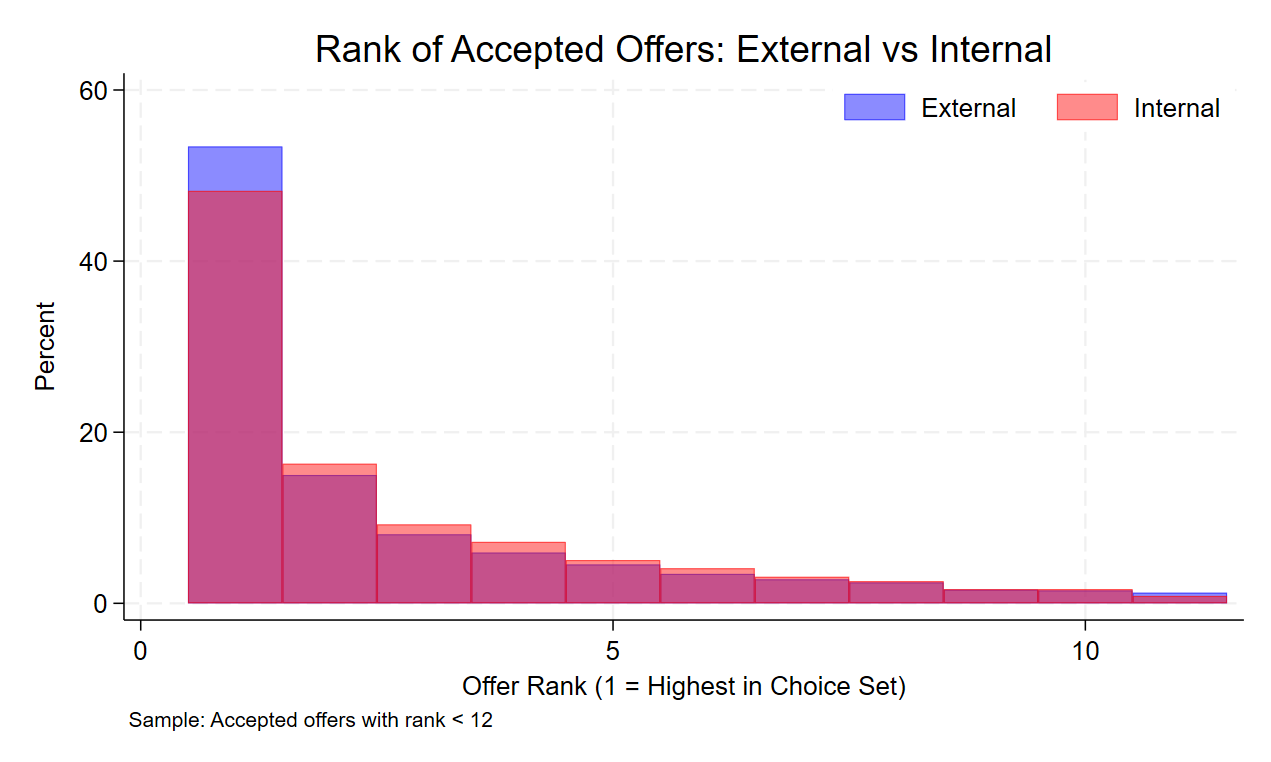
\includegraphics[scale=0.27]{../figures/IE4/IE4_rank_of_accepted_external.png} 
\end{tabular}
\end{figure} 


Distribution tests for offer ranks:
Wilcoxon rank-sum: z =  5.490, p = 0.0000



\begin{table}[htbp]\centering
\def\sym#1{\ifmmode^{#1}\else\(^{#1}\)\fi}
\caption{Rank Comparison: External vs Internal Accepted Offers}
\begin{tabular}{l*{1}{cccc}}
\hline\hline
            &        mean&         p50&          sd&       count\\
\hline
External    &            &            &            &            \\
offer\_rank  &        2.90&         1.0&        3.18&       13683\\
offer\_rank\_pct&       14.74&         0.0&       21.98&       13666\\
\hline
Internal    &            &            &            &            \\
offer\_rank  &        2.98&         2.0&        3.11&        4609\\
offer\_rank\_pct&       19.82&         8.3&       26.81&        4438\\
\hline
Total       &            &            &            &            \\
offer\_rank  &        2.92&         1.0&        3.17&       18292\\
offer\_rank\_pct&       15.98&         0.0&       23.36&       18104\\
\hline
\(N\)       &       18292&            &            &            \\
\hline\hline
\end{tabular}
\end{table}


Table 13 shows that
\begin{table}[htbp]\centering
\def\sym#1{\ifmmode^{#1}\else\(^{#1}\)\fi}
\caption{Share of Accepted Offers in Top Rankings}
\begin{tabular}{l*{6}{c}}
\hline\hline
            &        mean&        mean&        mean&        mean&        mean&        mean\\
\hline
\hline
\(N\)       &       18292&       18292&       18292&       18292&       18292&        8342\\
\hline\hline
\end{tabular}
\end{table}




  \begin{figure}[H]
\caption{}
 \label{fig:ie4_11}
\centering{}%
\begin{tabular}{cc}
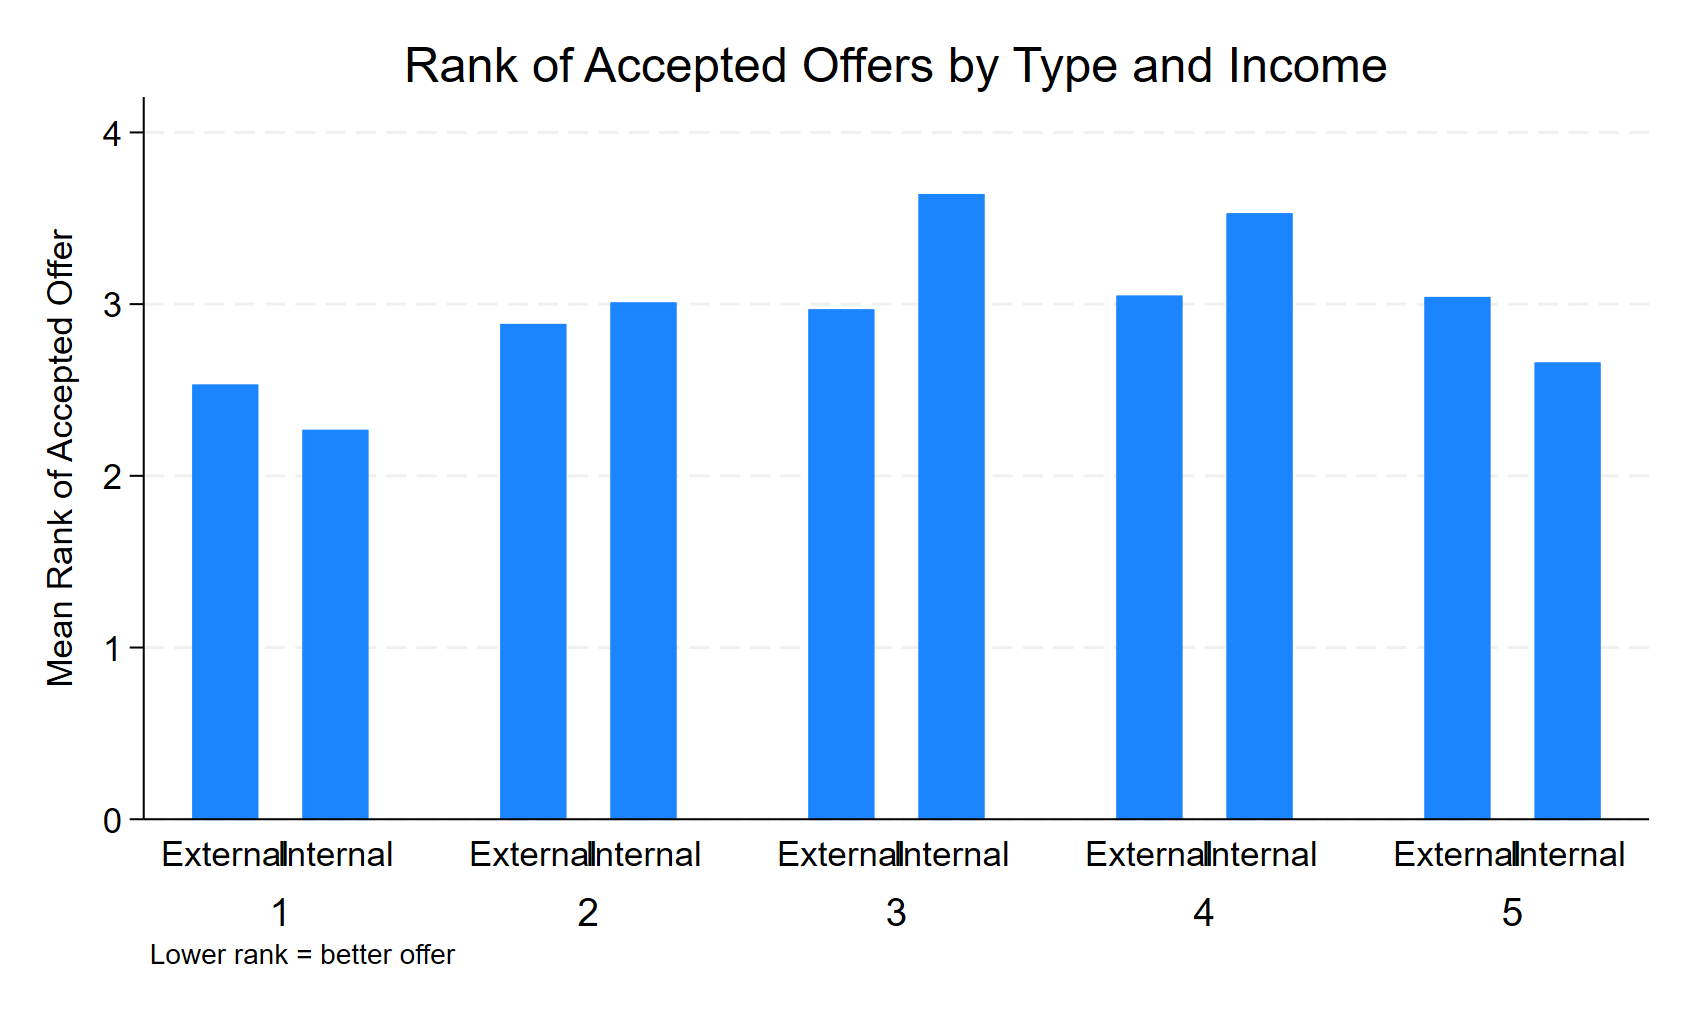
\includegraphics[scale=0.17]{../figures/IE4/IE4_rank_by_type_income.png} 
\end{tabular}
\end{figure} 

\newpage
A
\newpage
\subsection{Mortality and survival rates}

Figure \ref{fig:ie4_12} shows the mortality curves for the biggest firm. 

\begin{figure}[H]
\caption{}
\label{fig:ie4_12}
\centering{}%
\begin{tabular}{cc}
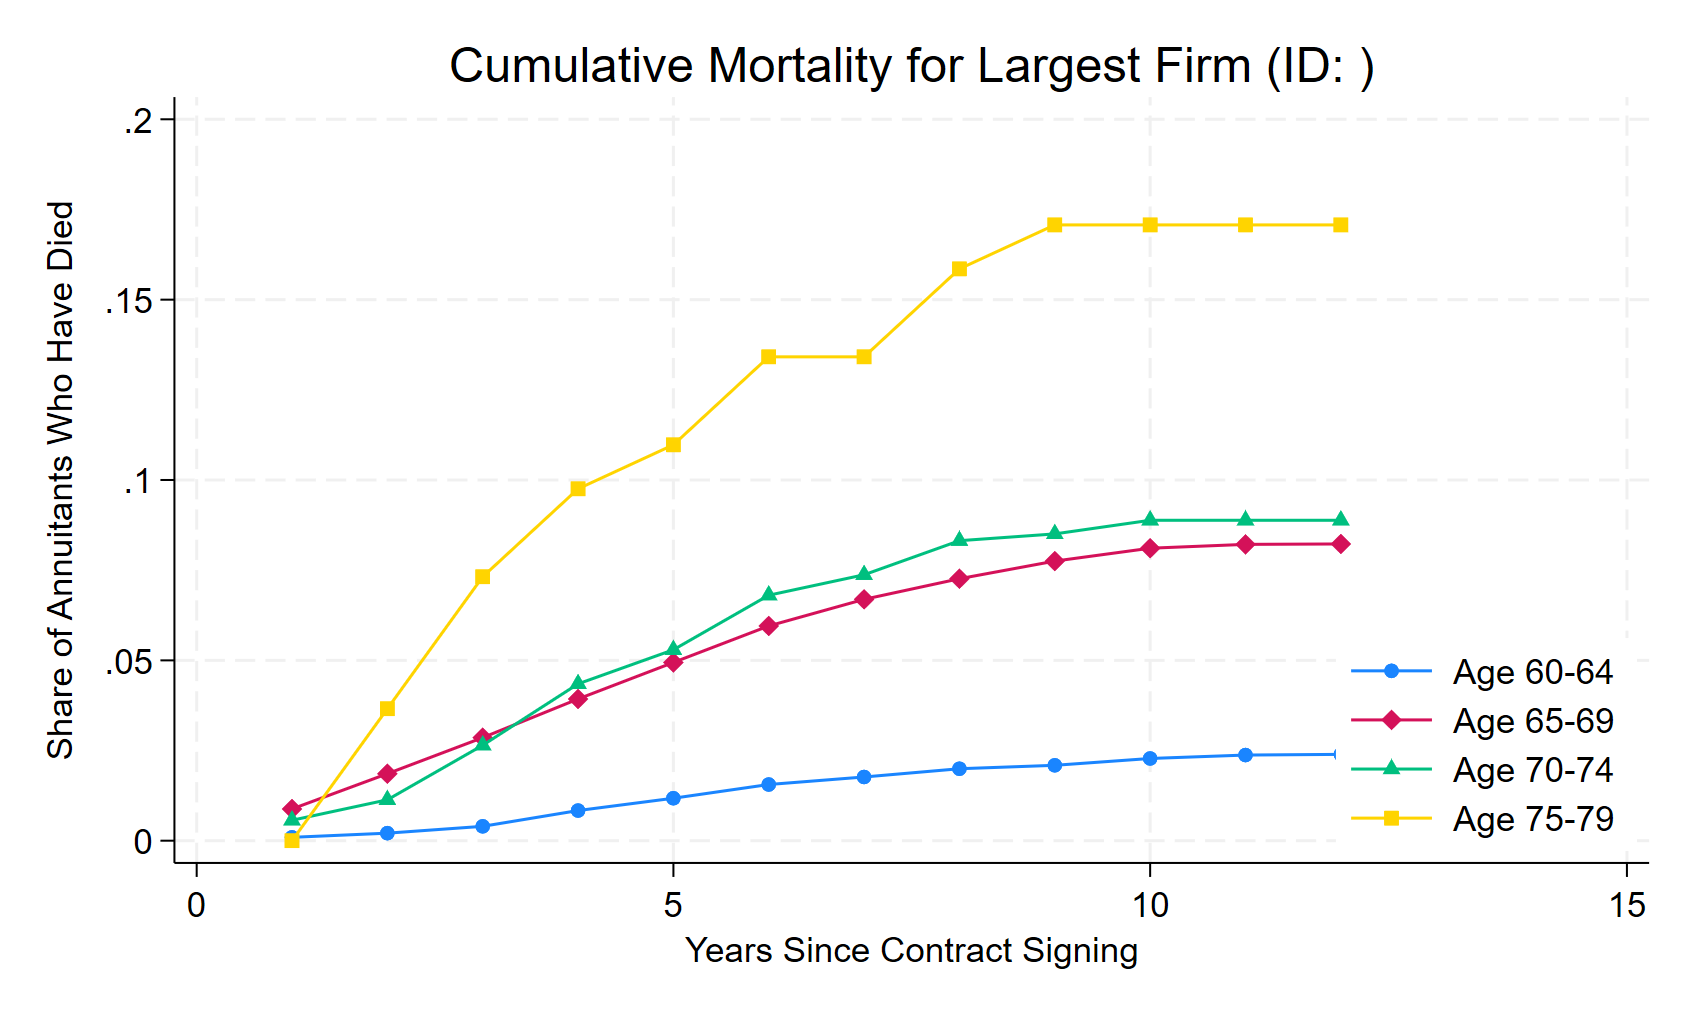
\includegraphics[scale=0.2]{../figures/IE4/IE4_mortality_curves_by_age.png} 
\end{tabular}
\end{figure} 

\subsection{Mortality and survival rates}


  
Figure \ref{fig:ie4_13} shows the share of individuals at each age that die. The left panel is unshmoothed and the right panel is smoothed. We can see that some firms have consistently lower mortalities (e.g. firm2). 

Figure \ref{fig:ie4_14} shows the survival curves for the same firms, where we can see that the survival rates vary across firms.
\begin{figure}[H]
\caption{}
\label{fig:ie4_13}
\centering{}%
\begin{tabular}{cc}
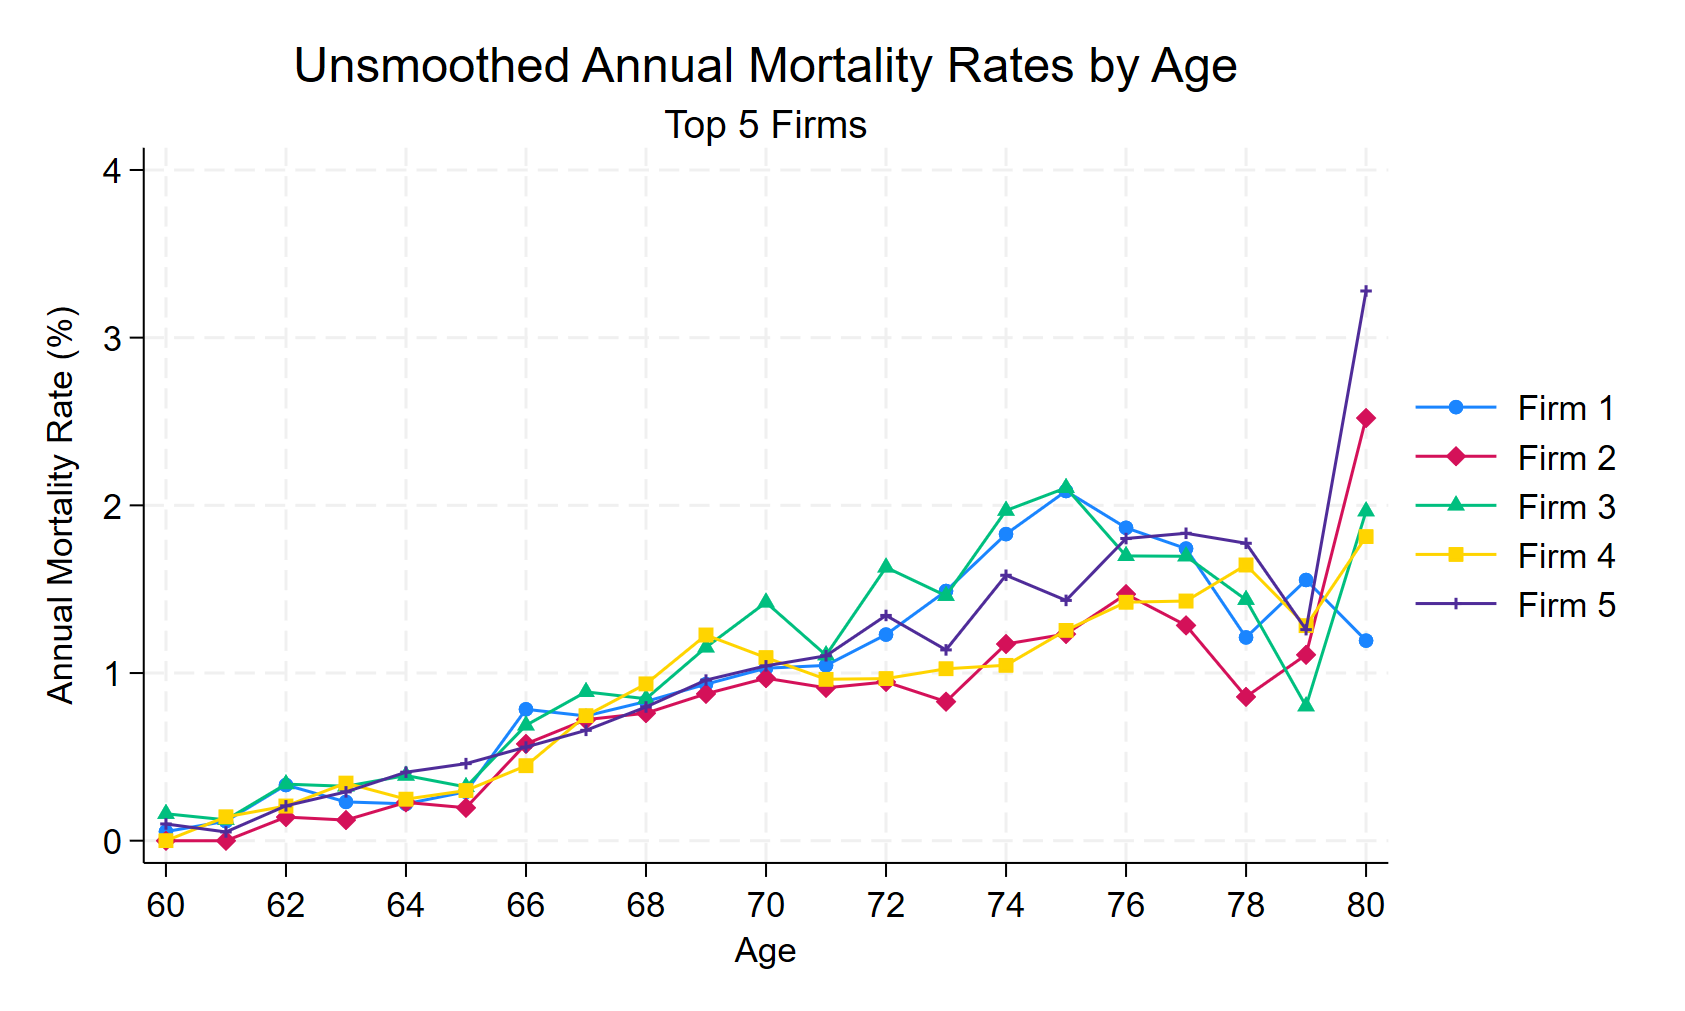
\includegraphics[scale=0.17]{../figures/IE4/IE4_mortality_rates_unsmoothed.png} 
& 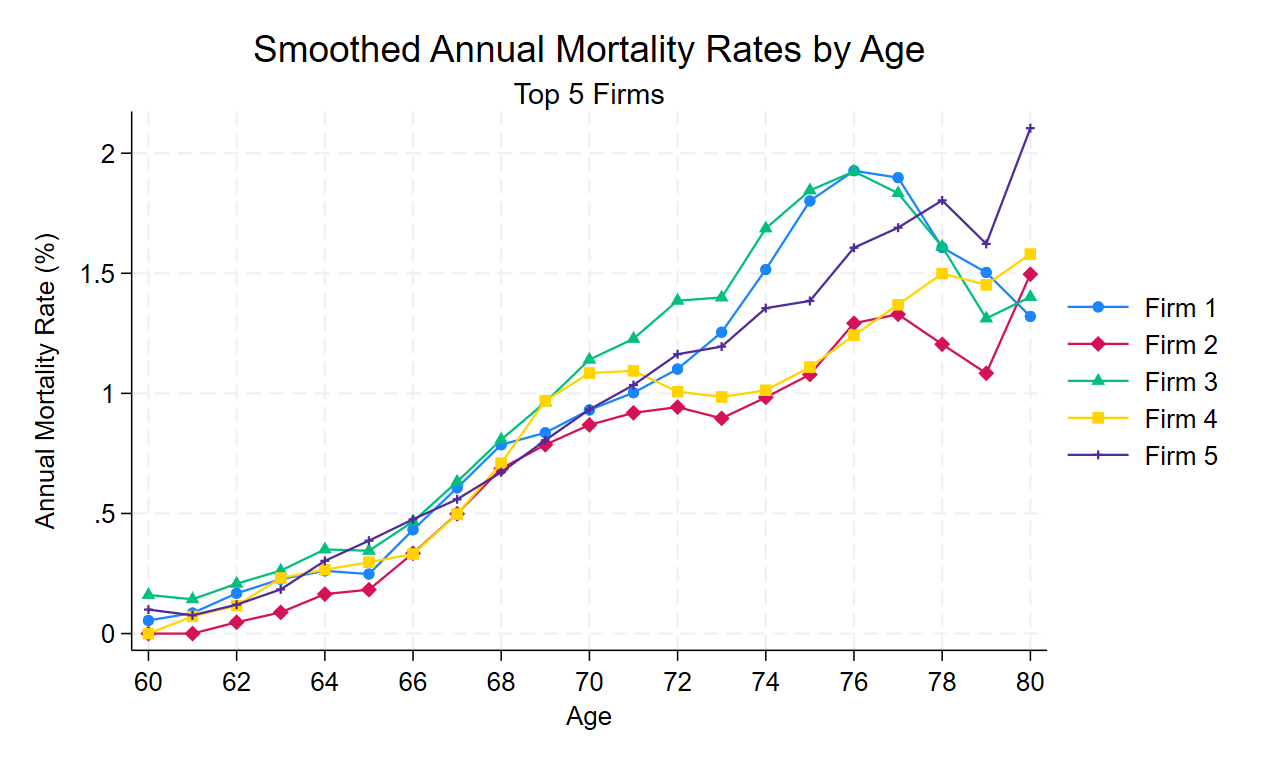
\includegraphics[scale=0.17]{../figures/IE4/IE4_mortality_rates_smoothed.png} 
\end{tabular}
\end{figure} 
 
The tables below use different tests to see whether the survival curves are statistically different across firms. We can reject the null hypothesis that they are the same. The first table uses the full sample and the second table uses the sample of men. 

 
  \begin{figure}[H]
\caption{}
 \label{fig:ie4_14}
\centering{}%
\begin{tabular}{cc}
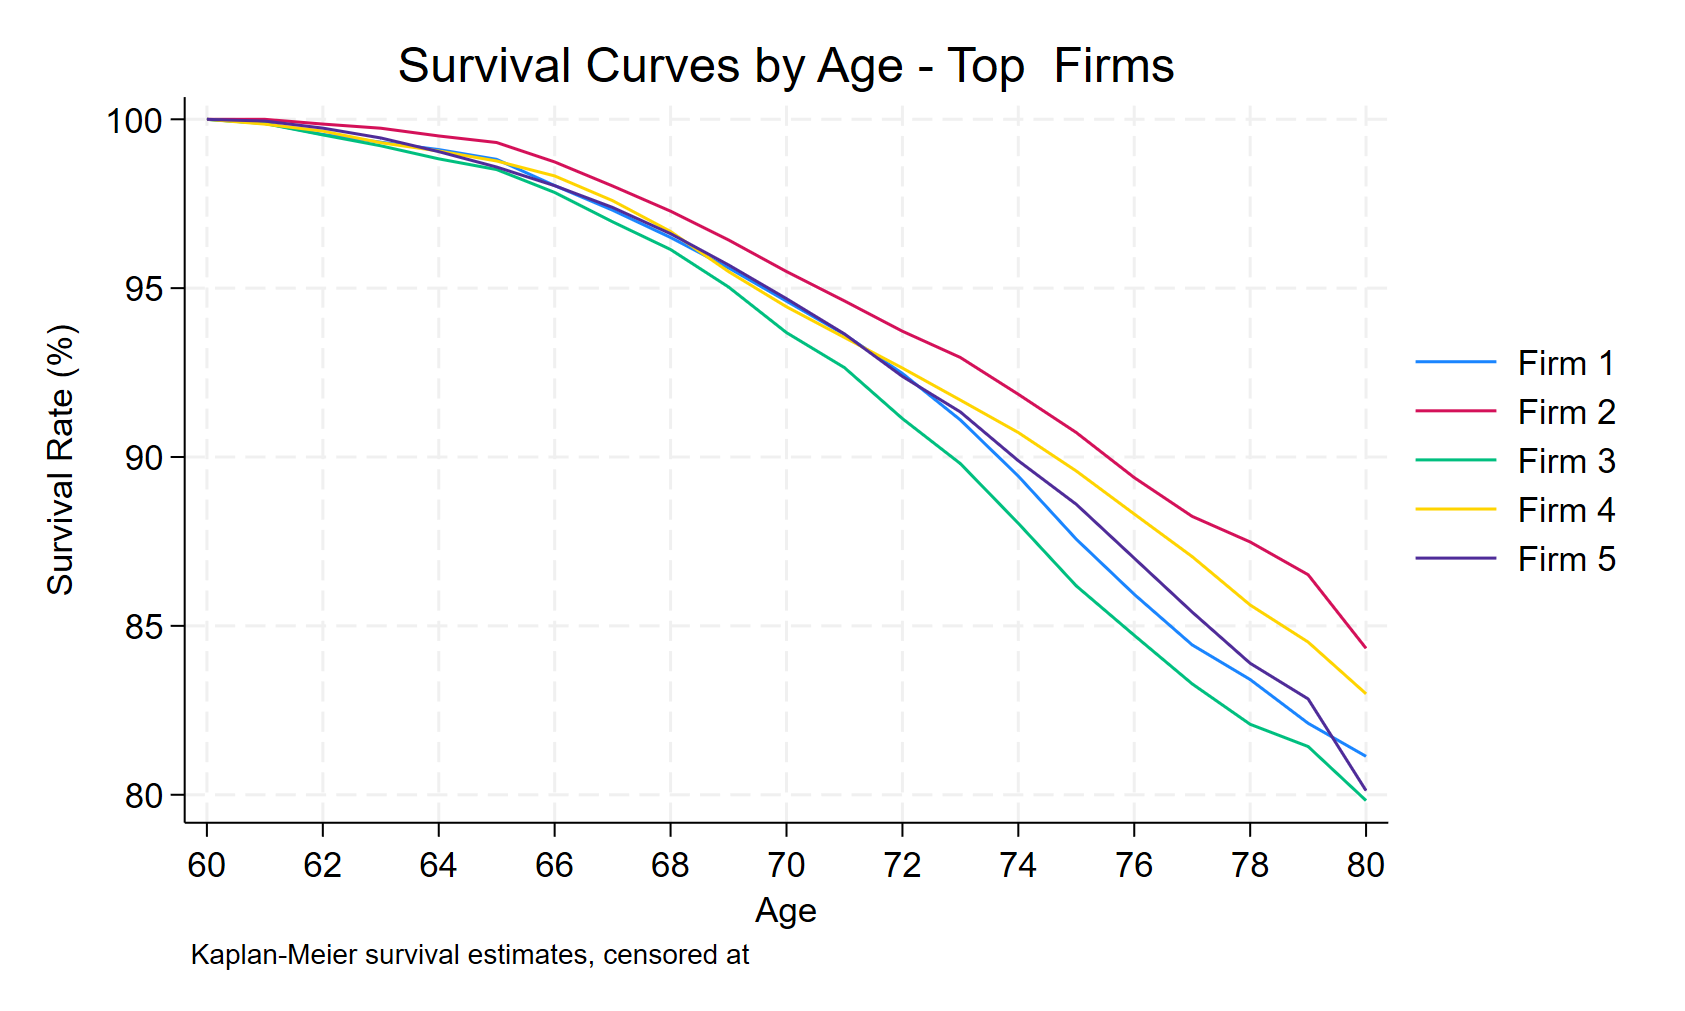
\includegraphics[scale=0.2]{../figures/IE4/IE4_survival_curves_by_age_top_firms.png} 
\end{tabular}
\end{figure} 

\begin{figure}[H]
\caption{}
\label{fig:ie4_15}
\centering{}%
\begin{tabular}{cc}
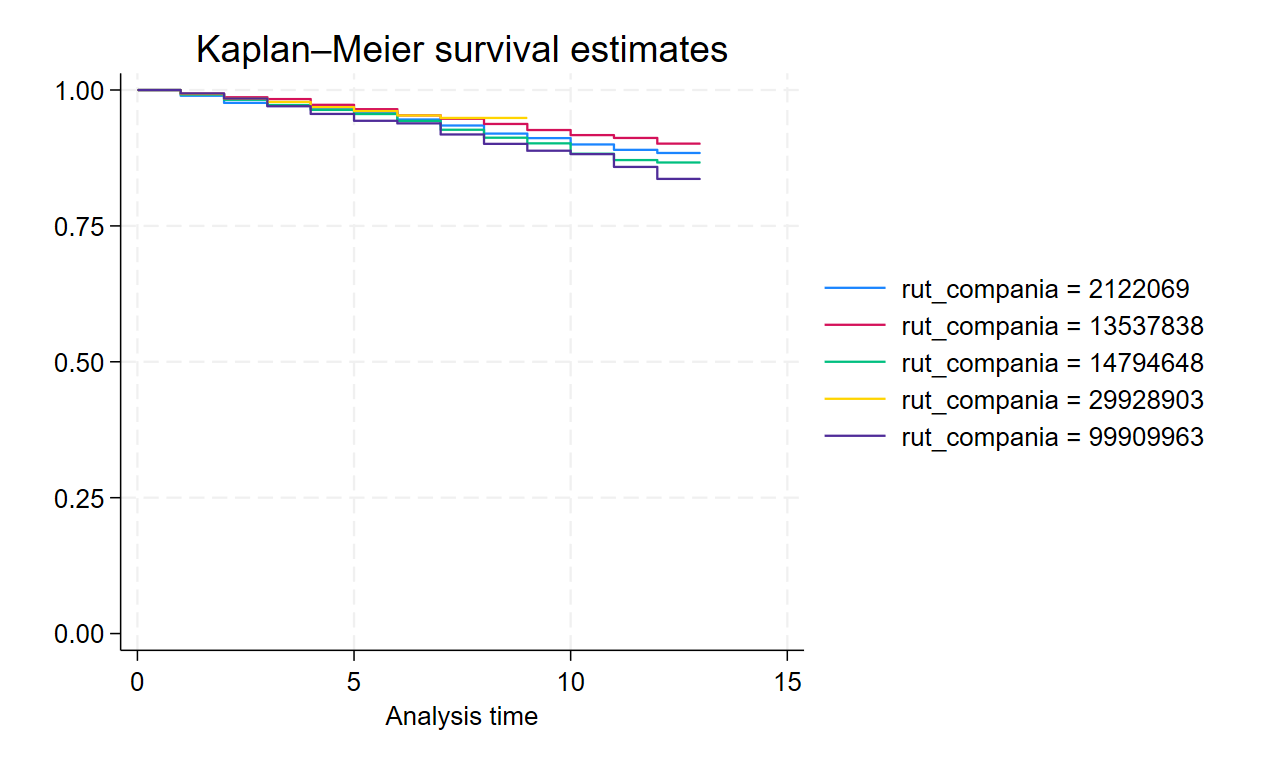
\includegraphics[scale=0.217]{../figures/IE4/IE4_km_curves_by_firm.png} 
& 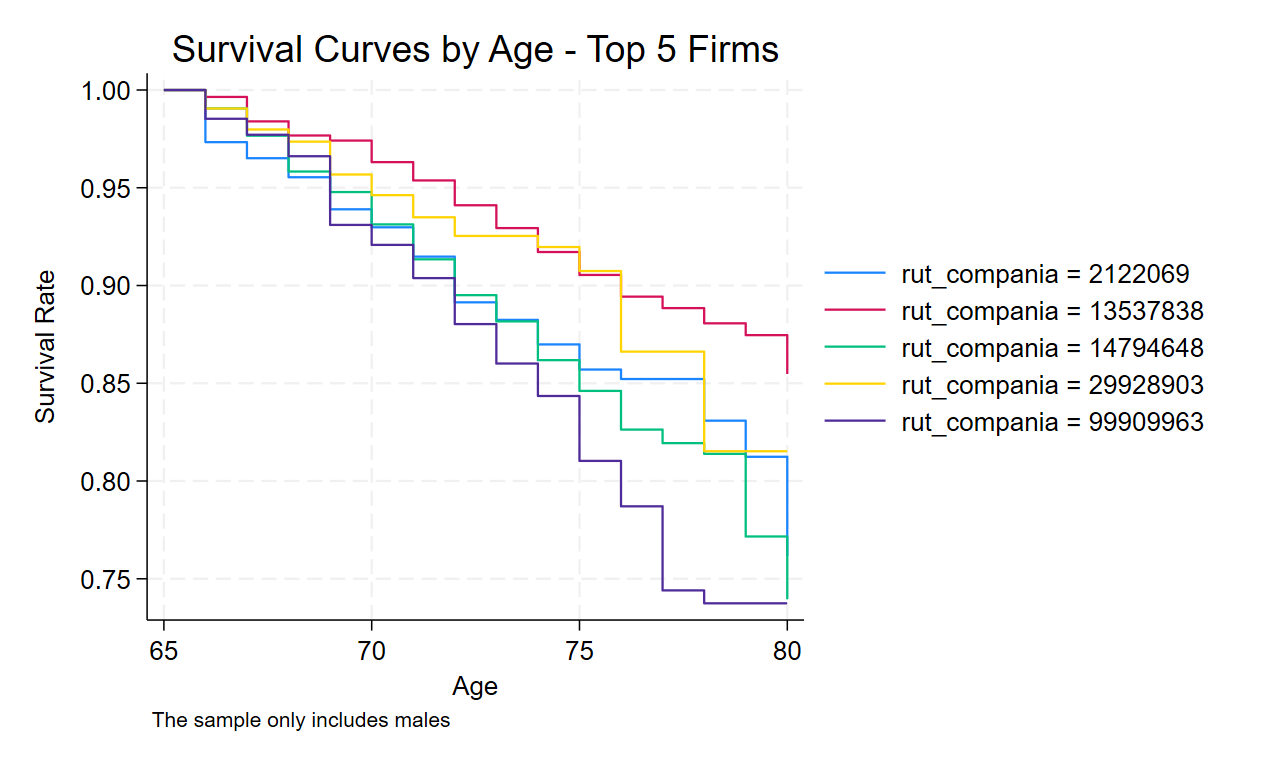
\includegraphics[scale=0.217]{../figures/IE4/IE4_km_curves_by_firm_males.png} 
\end{tabular}
\end{figure} 
 



\begin{table}[htbp]\centering
\caption{Equality of Survival Functions Tests}
\begin{tabular}{l*{3}{c}}
\hline\hline
            &       tests&            &            \\
            &        Chi2&     P-value&          df\\
\hline
Log-rank    &      19.798&      0.0005&           4\\
Wilcoxon    &      14.415&      0.0061&           4\\
Stratified\_LR&      13.937&      0.0075&           4\\
\hline\hline
\multicolumn{4}{l}{\footnotesize Log-rank test is sensitive to late differences}\\
\multicolumn{4}{l}{\footnotesize Wilcoxon test weights early times more heavily}\\
\multicolumn{4}{l}{\footnotesize Stratified log-rank adjusts for 5-year age groups}\\
\end{tabular}
\end{table}




\begin{table}[htbp]\centering
\caption{Equality of Survival Functions Tests}
\begin{tabular}{l*{3}{c}}
\hline\hline
            &       tests&            &            \\
            &        Chi2&     P-value&          df\\
\hline
Log-rank    &      30.609&      0.0000&           4\\
Wilcoxon    &      26.950&      0.0000&           4\\
Stratified\_LR&      23.175&      0.0001&           4\\
\hline\hline
\multicolumn{4}{l}{\footnotesize Sample only includes males.}\\
\multicolumn{4}{l}{\footnotesize Log-rank test is sensitive to late differences}\\
\multicolumn{4}{l}{\footnotesize Wilcoxon test weights early times more heavily}\\
\multicolumn{4}{l}{\footnotesize Stratified log-rank adjusts for 5-year age groups}\\
\end{tabular}
\end{table}


\end{document}